%  Manuscript for Applied Sciences (MDPI), article type: Review
%  Build:  latexmk -pdf manuscript.tex   (figures/ and tables/ are generated by scripts/*.py)
%  Lines marked "TODO(author)" must be completed or confirmed by the author before submission.
%=================================================================
\documentclass[applsci,review,submit,pdftex,oneauthor]{Definitions/mdpi}

%=================================================================
% MDPI internal commands - do not modify
\firstpage{1}
\makeatletter
\setcounter{page}{\@firstpage}
\makeatother
\pubvolume{1}
\issuenum{1}
\articlenumber{0}
\pubyear{2026}
\copyrightyear{2026}
\datereceived{ }
\daterevised{ }
\dateaccepted{ }
\datepublished{ }
\hreflink{https://doi.org/}

%=================================================================
\usepackage{longtable}
% Auto-generated by scripts/analysis.py from gallery/data.json -- do not edit by hand
\newcommand{\nModels}{215}
\newcommand{\nVLA}{135}
\newcommand{\nVA}{58}
\newcommand{\nOther}{22}
\newcommand{\nYC}{2}
\newcommand{\nYD}{14}
\newcommand{\nYE}{60}
\newcommand{\nYF}{91}
\newcommand{\nYG}{48}
\newcommand{\nManip}{111}
\newcommand{\nHum}{41}
\newcommand{\nMoMa}{34}
\newcommand{\nNav}{29}
\newcommand{\nInd}{74}
\newcommand{\nAcad}{66}
\newcommand{\nMixed}{73}
\newcommand{\nUnk}{2}
\newcommand{\nOpenYes}{100}
\newcommand{\nOpenPart}{17}
\newcommand{\nOpenNo}{59}
\newcommand{\nOpenUnk}{39}
\newcommand{\nHF}{89}
\newcommand{\nGH}{153}
\newcommand{\nPaper}{182}
\newcommand{\nReport}{3}
\newcommand{\nNoPaper}{30}
\newcommand{\nVerified}{145}
\newcommand{\nCorrected}{58}
\newcommand{\nUnverified}{12}
\newcommand{\nSecondary}{18}
\newcommand{\nDagger}{27}
\newcommand{\nParams}{113}
\newcommand{\medParams}{3.3}
\newcommand{\medParamsVLA}{5.0}
\newcommand{\nLLMsize}{81}
\newcommand{\medLLM}{4}
\newcommand{\nTGmodels}{109}
\newcommand{\nTGrecords}{145}
\newcommand{\nGPUh}{38}
\newcommand{\medGPUh}{1,856}
\newcommand{\qOneGPUh}{704}
\newcommand{\qThreeGPUh}{9,932}
\newcommand{\maxGPUh}{50,000}
\newcommand{\minGPUh}{24}
\newcommand{\rhoGpuhParams}{-0.18}
\newcommand{\nGpuhParams}{30}
\newcommand{\rhoGpuhDate}{0.16}
\newcommand{\rhoGpuhData}{0.64}
\newcommand{\nGpuhData}{12}
\newcommand{\nHz}{83}
\newcommand{\medHz}{20}
\newcommand{\nEst}{128}
\newcommand{\nAnchors}{38}
\newcommand{\nAnchorsValid}{37}
\newcommand{\nAnchorModels}{30}
\newcommand{\nAnchorDevices}{11}
\newcommand{\nDevices}{24}
\newcommand{\calMed}{1.37}
\newcommand{\calWithinTwo}{26}
\newcommand{\calWithinOneFive}{23}
\newcommand{\calBias}{0.95}
\newcommand{\looMed}{1.49}
\newcommand{\looWithinTwo}{23}
\newcommand{\nomMed}{2.99}
\newcommand{\nomWithinTwo}{7}
\newcommand{\trMed}{1.09}
\newcommand{\trN}{13}
\newcommand{\trWithinTwo}{11}
\newcommand{\refitMed}{1.29}
\newcommand{\nRLuse}{31}
\newcommand{\nRLpart}{28}
\newcommand{\nRLnone}{132}
\newcommand{\nRLund}{24}
\newcommand{\nMobile}{98}
\newcommand{\nAssess}{125}
\newcommand{\nNoSize}{78}
\newcommand{\nNoKind}{9}
\newcommand{\nNotAssessable}{87}
\newcommand{\nWeightsOpen}{123}
\newcommand{\nOpenHF}{6}
\newcommand{\nOpenEst}{89}
\newcommand{\memN}{23}
\newcommand{\memNbf}{18}
\newcommand{\memMed}{1.13}
\newcommand{\memWithinOneFive}{21}
\newcommand{\memWithinTwo}{23}
\newcommand{\memBias}{1.09}
\newcommand{\holdPred}{46}
\newcommand{\holdMeas}{43}
\newcommand{\refitBeta}{1}
\newcommand{\refitPhi}{0.5}
\newcommand{\refitCzero}{3}
\newcommand{\refitCt}{6}
\newcommand{\refitGamma}{1.75}


%=================================================================
\Title{Training and Deployment Resources of Robot Vision--Language--Action Models: A Review of 215 Models with a Validated Feasibility Estimator}

\TitleCitation{Training and Deployment Resources of Robot Vision--Language--Action Models: A Review of 215 Models with a Validated Feasibility Estimator}

% TODO(author): ORCID, name, affiliation, e-mail
\newcommand{\orcidauthorA}{0000-0000-0000-000X}
\Author{Firstname Lastname $^{1,}$*\orcidA{}}
\AuthorNames{Firstname Lastname}
\isAPAStyle{%
       \AuthorCitation{Lastname, F.}
         }{%
        \isChicagoStyle{%
        \AuthorCitation{Lastname, Firstname.}
        }{
        \AuthorCitation{Lastname, F.}
        }
}
\address[1]{%
$^{1}$ \quad Affiliation; yc424k@gmail.com}
\corres{Correspondence: yc424k@gmail.com}

%=================================================================
\abstract{Vision--language--action (VLA) models have become a common way to build general robot policies, but the resources they need---training compute, inference latency and memory---are reported unevenly, which makes it hard to match a model to a robot computer or a training budget. We review \nModels{} robot policy models released between October 2022 and October 2026 for manipulation, humanoid whole-body control, mobile manipulation and navigation. Each model was coded from primary sources into a 28-field schema with explicit labels for undisclosed and unverified values, and re-checked in a verification pass. Action heads shifted from discrete tokens to flow matching, and Qwen replaced Llama as the most common language backbone. Only \nGPUh{} models (18\%) report enough to compute training GPU-hours and 28 (13\%) report inference memory; industry-only models disclose their training hardware less often than other teams (19\% vs.\ 63\%). We propose a roofline-based estimator of inference latency, memory and fine-tuning cost that models token decoding and iterative denoising. Calibrated on \nAnchorsValid{} published latency measurements from \nAnchorDevices{} devices, it reaches a median error of \calMed$\times$ (\looMed$\times$ in leave-one-out validation). We use it to map which models can run at 10~Hz on eleven devices, from Jetson modules to an H100, and close with a ten-item reporting checklist.}

\keyword{vision--language--action models; robot foundation models; embodied AI; training compute; edge deployment; inference latency; roofline model; reporting standards; humanoid robots; mobile manipulation}

\featuredapplication{The open dataset and estimator let robot developers check, before downloading or training anything, whether a published VLA model fits the memory and control-rate budget of their onboard computer and how much GPU memory fine-tuning it will need.}

\begin{document}

%%%%%%%%%%%%%%%%%%%%%%%%%%%%%%%%%%%%%%%%%%
\section{Introduction}

Robot learning has converged on a recipe borrowed from language and vision: pretrain a large network on heterogeneous data, then adapt it to a robot and a task. Vision--language--action (VLA) models apply this recipe to control. They attach an action-generating head to a vision--language model (VLM), so that one network maps camera images and a language instruction to robot actions~\cite{ax230715818,ax240609246,ax241024164}. Since RT-2~\cite{ax230715818} showed in 2023 that web-scale VLM pretraining transfers to robot control, VLAs have spread from tabletop manipulation to humanoid whole-body control~\cite{ax250314734,web-figure-helix}, mobile manipulation~\cite{ax250416054,ax250313446} and navigation~\cite{ax241204453,ax241206224}. Academic laboratories and companies now release several such models per month (Figure~\ref{fig:composition}a).

For anyone who wants to use one of these models, the first questions are practical. Will the model fit in the memory of the robot's onboard computer? Will it produce actions fast enough for the task? Can it be fine-tuned on the GPUs at hand, and what did it cost to pretrain? The answers depend on a handful of quantities---parameter counts, accelerator-hours, inference latency on a named device, peak memory---that are scattered across papers, model cards, repositories and blog posts, are reported in inconsistent units, or are not reported at all. Existing surveys organise the field by architecture and training paradigm~\cite{ma2024survey,sapkota2025,zhong2025token,shao2025,kawaharazuka2025vla}, by efficiency technique~\cite{guan2025efficient,yu2025efficient}, by the barriers to deployment at the edge~\cite{grover2026edge}, or by data and benchmarks~\cite{wang2026data}. They explain how VLAs work and how they might be made cheaper. They do not tell a reader how much a specific model costs to train or whether it will run on a specific device, and they do not measure how often the required numbers are missing.

This review takes a resource-centred view of the field. We coded \nModels{} robot policy models released between October 2022 and October 2026 against a fixed schema drawn from primary sources, labelled every missing or uncertain value explicitly, and re-checked each record in a verification pass. On this corpus we make four contributions:
\begin{enumerate}
\item An open, evidence-labelled dataset of \nModels{} models (\nVLA{} VLAs, \nVA{} visuomotor policies without a pretrained VLM and \nOther{} related systems) covering manipulation, humanoid whole-body control, mobile manipulation and navigation, with \nTGrecords{} per-stage training-hardware records, \nAnchors{} published latency measurements and a control-interface taxonomy for \nMobile{} mobile robots. The dataset is also published as an interactive gallery.
\item A quantitative synthesis of architecture and resource trends: the shift of action heads from discrete tokens to flow matching, the shift of language backbones from Llama to Qwen, model size, training compute and data, control rates, and where reinforcement learning (RL) enters the pipeline.
\item A disclosure audit of twelve resource items, which shows which numbers are reported, which are not, and how reporting differs between industry and academic teams.
\item A roofline-based estimator of inference latency, memory and fine-tuning cost, calibrated on the published measurements and validated by leave-one-out prediction, which we use to map how many models can run at 10~Hz on eleven devices from Jetson modules to an H100.
\end{enumerate}
We end with a ten-item checklist for reporting the resources of robot foundation models.

Section~\ref{sec:related} positions this review against prior surveys. Section~\ref{sec:methods} describes how the corpus was built and coded. Sections~\ref{sec:corpus}--\ref{sec:training} present the corpus, architecture trends and training resources. Section~\ref{sec:disclosure} reports the disclosure audit. Section~\ref{sec:estimator} presents the estimator and the feasibility maps. Sections~\ref{sec:rl} and \ref{sec:base} cover reinforcement learning and mobile-base control. Section~\ref{sec:discussion} discusses implications and limitations, and Section~\ref{sec:conclusions} concludes.

%%%%%%%%%%%%%%%%%%%%%%%%%%%%%%%%%%%%%%%%%%
\section{Related Surveys}\label{sec:related}

Early surveys of foundation models in robotics~\cite{firoozi2023,hu2023toward,kawaharazuka2024real} predate most of the models in our corpus. They name real-time execution and compute as open challenges but do not quantify them. Surveys dedicated to VLAs~\cite{ma2024survey,adilkhanov2025,sapkota2025,zhong2025token,din2025,shao2025,li2025survey,zhang2025pure,kawaharazuka2025vla} organise the literature by component (vision encoder, language backbone, action decoder), by action representation~\cite{zhong2025token} or by training paradigm, and several discuss efficiency in qualitative terms. Two recent surveys make efficiency their subject. Guan et al.~\cite{guan2025efficient} group techniques for reducing latency, memory and training cost into model architecture, perception features, action generation and training or inference strategies, and Yu et al.~\cite{yu2025efficient} organise efficient-VLA methods across the model, training and data pipeline. Grover et al.~\cite{grover2026edge} analyse the constraints of running embodied foundation models on edge hardware and argue that autoregressive VLAs are limited mainly by memory bandwidth and diffusion-based controllers by compute, a view that our estimator formalises and tests against measurements. Other surveys cover datasets and benchmarks~\cite{wang2026data}, world--action models~\cite{shen2026wam,lu2026wam}, foundation models for mobile service robots~\cite{lisondra2025} and VLAs for aerial robots and bimanual manipulation~\cite{sa2026drones}.

Table~\ref{tab:surveys} summarises the focus of these surveys as stated by their authors. Prior surveys describe methods; this review treats resources as data. Judging from their stated scope, none of the surveys above codes per-model training hardware, inference latency and memory under explicit evidence labels, measures how often these values are disclosed, or validates a predictive latency model against published measurements.

\begin{table}[H]
\caption{Recent surveys related to VLA models and the focus stated in their abstracts.\label{tab:surveys}}
\small
\begin{tabularx}{\textwidth}{@{}l c X@{}}
\toprule
\textbf{Survey} & \textbf{Year} & \textbf{Stated focus}\\
\midrule
Firoozi et al.~\cite{firoozi2023} & 2023 & Foundation models across the robot autonomy stack\\
Hu et al.~\cite{hu2023toward} & 2023 & Foundation models for general-purpose robots; meta-analysis\\
Ma et al.~\cite{ma2024survey} & 2024 & VLA taxonomy: components, low-level control policies, high-level task planners\\
Sapkota et al.~\cite{sapkota2025} & 2025 & Concepts, progress, applications and challenges (over 80 VLA models)\\
Zhong et al.~\cite{zhong2025token} & 2025 & VLAs viewed through action tokenization\\
Shao et al.~\cite{shao2025} & 2025 & Large-VLM-based VLAs for robotic manipulation\\
Kawaharazuka et al.~\cite{kawaharazuka2025vla} & 2025 & Full-stack review, including hardware, towards real-world applications\\
Guan et al.~\cite{guan2025efficient} & 2025 & Efficiency techniques for embodied manipulation\\
Yu et al.~\cite{yu2025efficient} & 2025 & Efficient VLAs across the model, training and data pipeline\\
Grover et al.~\cite{grover2026edge} & 2026 & Deployment constraints of embodied foundation models at the edge\\
Wang et al.~\cite{wang2026data} & 2026 & Datasets, benchmarks and data engines\\
Sa et al.~\cite{sa2026drones} & 2026 & VLAs for aerial robots and bimanual manipulation (183 contributions)\\
\midrule
This review & 2026 & Training and deployment resources of \nModels{} models in four domains; disclosure audit; latency, memory and fine-tuning estimator validated on published measurements\\
\bottomrule
\end{tabularx}
\end{table}

%%%%%%%%%%%%%%%%%%%%%%%%%%%%%%%%%%%%%%%%%%
\section{Materials and Methods}\label{sec:methods}

\subsection{Scope and Inclusion Criteria}

We included models first described between January 2022 and 19 October 2026 that map visual observations, optionally together with language and proprioception, to robot actions or to commands consumed by a robot controller, in one of four domains: manipulation, humanoid whole-body control, mobile manipulation and navigation. Each model was assigned one of three types.
\begin{itemize}
\item \textbf{VLA} (\nVLA{} models): policies built on a pretrained VLM or language model, or presented by their authors as VLAs.
\item \textbf{VA} (\nVA{} models): visuomotor policies trained without a pretrained VLM, such as ACT~\cite{ax230413705} and Diffusion Policy~\cite{ax230304137}. They are included as reference points because many VLAs reuse their action heads and because several remain strong baselines.
\item \textbf{Other} (\nOther{} models): systems that are not single end-to-end policies but shape VLA practice, such as world--action models that predict future video and actions~\cite{ax260116163,ax260215922}, embodied-reasoning VLMs that direct a VLA~\cite{ax250320020}, inference-time techniques such as real-time chunking~\cite{ax250607339}, and fleet data-collection systems~\cite{ax240112963}.
\end{itemize}
The release date is the month of the first public description (paper, blog post or model card).

\subsection{Identification of Models}

% TODO(author): describe how candidates were found. The sentence below is a placeholder that must match what was actually done.
Candidate models were collected from [TODO(author): e.g., the reference lists of prior surveys, arXiv cs.RO listings, and announcements by robotics companies and laboratories]. The corpus was assembled in three rounds with reference dates of 6 October 2026 (165 models, mostly manipulation and humanoid models), 14 October 2026 (46 mobile-manipulation and navigation models) and 19 October 2026 (four further releases). Values were coded as they stood on the reference date of each round.

\subsection{Data Extraction}

For each model, the 28 fields in Table~\ref{tab:schema} were filled from primary sources: the arXiv paper, the README of the official repository, the model card, or the developer's official blog post. Names of models, datasets and hardware were kept as written in the source. Three fields were also parsed as numbers for analysis: total parameters (billions), pretraining GPU/TPU-hours and data hours.

\begin{table}[H]
\caption{The 28-field extraction schema.\label{tab:schema}}
\small
\begin{tabularx}{\textwidth}{@{}l X@{}}
\toprule
\textbf{Group} & \textbf{Fields}\\
\midrule
Identity & Model; group; type (VLA, VA, other); domain; release date; organisations; weights released\\
Architecture & Architecture; backbone and action representation; key features (two sentences); parameters (as reported); parameters (billions)\\
Training & Pretraining accelerator; pretraining duration; pretraining steps and batch; pretraining GPU/TPU-hours; basis and unit of the hours; fine-tuning accelerator and duration\\
Data and evaluation & Tasks and benchmarks; robots and embodiments; data type; data scale; data hours; main datasets\\
Inference & Inference device, rate, latency and memory as reported\\
Provenance & Notes; verification status; primary source URL\\
\bottomrule
\end{tabularx}
\end{table}

A second set of fields was coded from the same sources: the vision encoder; the language backbone and its family; the action head and its family (11 classes); action-chunk length; control rate; where inference runs (onboard, local PC, remote server or cloud); inference memory; whether and where RL is used (four statuses and six categories); the type of mobile base and the interface through which the policy commands it (eight classes); and links to official code and weight repositories. Training hardware was further normalised into per-stage records (stage, accelerator model, count, duration and the source's wording) for \nTGmodels{} models, giving \nTGrecords{} records.

\subsection{Evidence Rules}

Two labels distinguish missing values. ``Not disclosed'' means that no primary source reports the value; ``unverified'' means that the original could not be checked. Missing values were never estimated, with one exception: pretraining GPU-hours were computed as accelerator count times duration when both were reported as numbers. Values available only from secondary sources such as news articles or third-party papers were kept but marked (\nSecondary{} records contain at least one such value), values not checked against the original were marked separately (\nDagger{} records), and conflicting values from different primary sources were recorded side by side. Every field keeps a link to its source.

\subsection{Verification}

Each record was then checked against its primary sources in a second, independent pass. Of the \nModels{} records, \nVerified{} were confirmed unchanged, \nCorrected{} were corrected, and \nUnverified{} could not be fully verified (11 were not re-checked and one has no primary source). The verification status is stored with every record.

\subsection{Derived Variables and Analysis}

Models were grouped into four macro-domains from their coded domain (manipulation, humanoid, mobile manipulation including legged mobile manipulators, and navigation). Developers were grouped by affiliation into industry-only (\nInd{} models), academic-only (\nAcad{}) and mixed teams (\nMixed{}); public research institutes and non-profit laboratories (for example, Shanghai AI Laboratory, BAAI and the Allen Institute for AI) count as academic and corporate research laboratories (for example, Google DeepMind, NVIDIA, Microsoft Research and Toyota Research Institute) as industry; two models with no stated affiliation were left unclassified.

For the disclosure audit (Section~\ref{sec:disclosure}) we scored twelve items per model as disclosed or not: total parameter count; backbone (V)LM, including an explicit statement that there is none; action-head type; training accelerator model for at least one stage; training duration for at least one stage; pretraining GPU/TPU-hours, reported or computable; amount of training data; control rate; inference device; inference memory; released weights (full or partial); and an official code repository. Differences between industry-only models and all other models were tested with Fisher's exact test and Holm's correction across the twelve items. We report medians and interquartile ranges, and rank correlations as Spearman's $\rho$. All numbers, tables and figures in this article are produced by scripts that read the released dataset directly.

\subsection{Use of Generative AI}

% TODO(author): MDPI requires an accurate description. Edit to match exactly how GenAI was used for data collection and verification.
Generative AI was used in this work as follows: [TODO(author): describe any use in locating sources and extracting or verifying values]. A generative AI assistant (Claude, Anthropic) was also used to write the analysis and plotting scripts and to draft the text of this manuscript. All analyses were run on the released dataset, and the author reviewed and edited all text and takes full responsibility for the content.

%%%%%%%%%%%%%%%%%%%%%%%%%%%%%%%%%%%%%%%%%%
\section{The Corpus}\label{sec:corpus}

Figure~\ref{fig:anatomy} shows the anatomy that the schema follows. A VLA encodes one or more camera views, passes the visual tokens and the instruction through a (V)LM backbone, and decodes actions with a head; the head either emits discrete tokens one at a time, runs several denoising passes of a smaller network, or predicts actions in one forward pass. Many systems, especially humanoids and legged robots, add a low-level controller that turns the policy's output into joint commands.

\begin{figure}[H]
\begin{adjustwidth}{-\extralength}{0cm}
\centering
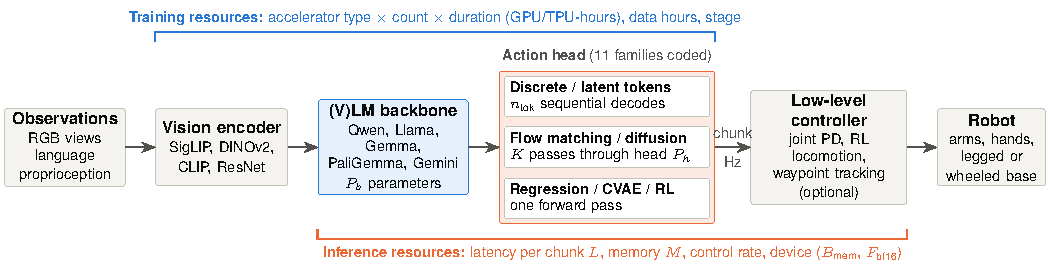
\includegraphics[width=\linewidth]{figures/fig1_anatomy}
\end{adjustwidth}
\caption{Anatomy of a VLA system and the resources coded in this review. Training resources cover the vision encoder, backbone and action head; inference resources span the backbone, the action head and any low-level controller. The symbols are those of the estimator in Section~\ref{sec:estimator}.\label{fig:anatomy}}
\end{figure}

The corpus grows from \nYC{} models in 2022 and \nYD{} in 2023 to \nYE{} in 2024 and \nYF{} in 2025; \nYG{} models appeared in 2026 up to the cut-off of 19 October (Figure~\ref{fig:composition}a). Manipulation accounts for \nManip{} models, humanoid whole-body control for \nHum{}, mobile manipulation for \nMoMa{} and navigation for \nNav{}. Industry-only teams released \nInd{} models, academic-only teams \nAcad{} and mixed teams \nMixed{}.

\begin{figure}[H]
\begin{adjustwidth}{-\extralength}{0cm}
\centering
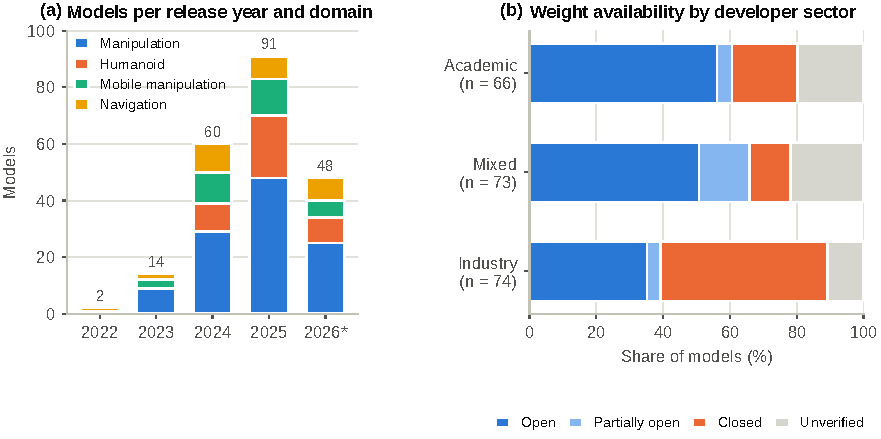
\includegraphics[width=\linewidth]{figures/fig2_composition}
\end{adjustwidth}
\caption{Composition of the corpus. (\textbf{a}) Models per release year and domain (*2026 up to 19 October). (\textbf{b}) Weight availability by developer sector.\label{fig:composition}}
\end{figure}

Most models are documented by a paper: \nPaper{} records cite an arXiv paper (176 distinct preprints, since some papers describe two models), \nReport{} cite a technical report, and \nNoPaper{} are documented only on the web, through blog posts, model cards, repositories or, in one case, news articles. Web-only documentation is concentrated in industry: 29 of the 74 industry-only models (39\%) have no paper or report, against one of the 66 academic-only models. Weights are fully released for \nOpenYes{} models and partially for \nOpenPart{}, withheld for \nOpenNo{}, and could not be verified for \nOpenUnk{}. \nHF{} models have weights on Hugging Face and \nGH{} have an official code repository. Openness also follows the developer: 61\% of academic-only and 66\% of mixed-team models release weights at least partially, against 39\% of industry-only models; half of the industry-only models (37 of 74) are closed (Figure~\ref{fig:composition}b).

%%%%%%%%%%%%%%%%%%%%%%%%%%%%%%%%%%%%%%%%%%
\section{Architecture Trends}\label{sec:architecture}

\subsection{Action Heads}

The action head is where VLA designs have changed most (Figure~\ref{fig:architecture}a). Early VLAs followed RT-1 and RT-2 in discretising each action dimension into bins and decoding them as language tokens~\cite{ax221206817,ax230715818,ax240609246}. Discrete or latent-action tokens still made up 30\% of the models released in 2024 (18 of 60) but 21\% in 2025 (19 of 91) and 8\% in 2026 (4 of 48). Flow matching~\cite{lipman2023flow}, introduced to VLAs by $\pi_0$~\cite{ax241024164}, went the other way: one model in 2024, 18 in 2025 (20\%) and 17 in 2026 (35\%), when it became the most common disclosed head. Diffusion heads~\cite{ho2020ddpm}, popularised for visuomotor control by Diffusion Policy~\cite{ax230304137}, were common in 2024 (15 models) and rare in 2026 (one model). Across the whole corpus the head families are discrete tokens (41), flow matching (36), diffusion (33), regression (26), RL policies (18), hybrids of autoregressive and diffusion or flow decoding (9), video world models (7), latent actions (6), CVAE (4) and other (7); 28 models do not disclose the head. The undisclosed share grew from 3\% in 2024 to 33\% in 2026, a first sign of the reporting gap analysed in Section~\ref{sec:disclosure}.

\begin{figure}[H]
\begin{adjustwidth}{-\extralength}{0cm}
\centering
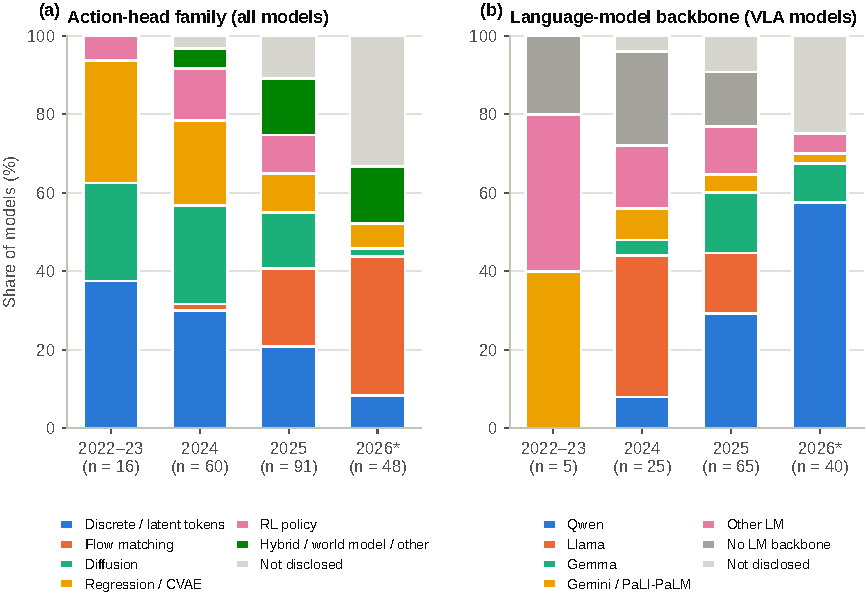
\includegraphics[width=\linewidth]{figures/fig3_architecture}
\end{adjustwidth}
\caption{Architecture trends by release year (*2026 up to 19 October). (\textbf{a}) Action-head family across all models. (\textbf{b}) Language-model family of the backbone among VLA models.\label{fig:architecture}}
\end{figure}

\subsection{Language Backbones}

Among the \nVLA{} VLAs, the Qwen family is the most common backbone (44 models), followed by Llama (19), Gemma including PaliGemma~\cite{beyer2024paligemma} (15), Gemini (5) and PaLI/PaLM (3); 16 use other language models (SmolLM, InternLM, Phi, Mamba and others), 16 condition on language through a separate text encoder without a language-model backbone (for example, RDT-1B~\cite{ax241007864}), and 17 do not disclose the backbone. The mix changed quickly (Figure~\ref{fig:architecture}b). In 2024, Llama-based backbones such as the Prismatic VLM~\cite{karamcheti2024prismatic} behind OpenVLA~\cite{ax240609246} accounted for 9 of 25 VLAs and Qwen for 2. In 2025 Qwen led with 19 of 65, and in 2026 it accounts for 23 of 40 VLAs while no new VLA in the corpus uses Llama. One likely driver is the availability of strong small Qwen VLMs~\cite{bai2025qwen25vl}, but the corpus cannot test this.

Where the size of the language model is reported (\nLLMsize{} models), the median is \medLLM{}B. The most common size is 7B (26 models), 42 models use 4B or less and five use 32B or more. Most models with a reported language-model size (68 of 81, nearly all of them VLAs) use 2--8.5B parameters, which matters for the memory analysis in Section~\ref{sec:estimator}.

\subsection{Model Size}

Total parameter counts are disclosed for \nParams{} models (median \medParams{}B; Figure~\ref{fig:size}). VLAs are much larger than visuomotor policies without a VLM (median 5B versus 0.093B). The yearly median rose from 0.0975B in 2022--2023 to 1.25B in 2024 and 4.1B in 2025, and stayed at 4.0B in 2026. The largest models are the 55B RT-2 variants~\cite{ax230715818,ax231008864,ax240301823} and the 72B DiVLA~\cite{ax241203293}, but no model released since January 2025 discloses more than 14B parameters. The plateau around 4B is consistent with designs that must run on a robot or a single GPU at control rates; it may also reflect that the largest proprietary models do not disclose their size.

\begin{figure}[H]
\centering
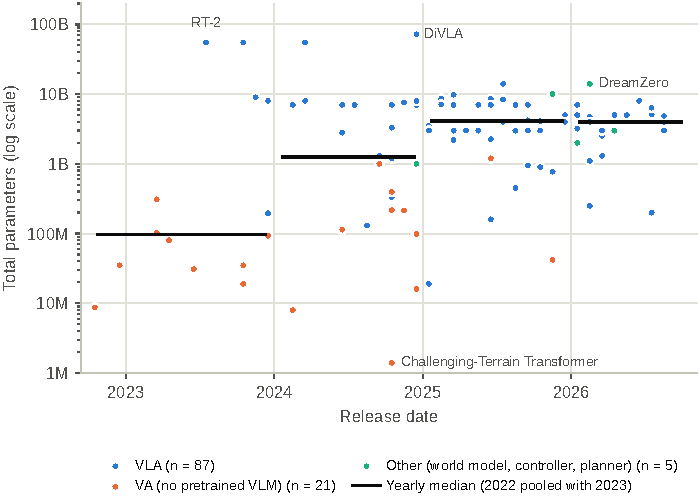
\includegraphics[width=\textwidth]{figures/fig4_size}
\caption{Total parameters against release date for the \nParams{} models that disclose them. Black segments mark the yearly median.\label{fig:size}}
\end{figure}

\subsection{Chunking, Control Rate and Hierarchy}

Of the models that describe their action output, 92 predict chunks of several future actions and 20 predict one step at a time; 103 do not say. Chunking decouples the control rate from inference latency: a policy that needs 70~ms per inference can still command the robot at 50~Hz by executing a 50-step chunk while the next one is computed~\cite{ax230413705,ax241024164,ax250607339}. Eighty-eight models report a control or execution rate (median 20~Hz among the 83 with a numeric value; 58 at 10~Hz or more). The rate depends on the head: models with discrete-token heads report a median of 3~Hz (11 models), against 10~Hz for diffusion (20), 30~Hz for flow matching (11) and 50~Hz for RL policies (13).

Hierarchy is the other route to speed. Forty-nine models document a multi-stage pipeline; 28 include a separate low-level controller and 28 include a VLM or LLM stage. Typical are dual-system designs in which a slow VLM runs at a few hertz and a small, fast action module runs at tens to hundreds of hertz: GR00T N1 pairs a 10~Hz VLM with a 120~Hz flow-matching transformer~\cite{ax250314734}, and Helix pairs a 7B VLM at 7--9~Hz with an 80M-parameter policy at 200~Hz~\cite{web-figure-helix}.

%%%%%%%%%%%%%%%%%%%%%%%%%%%%%%%%%%%%%%%%%%
\section{Training Resources}\label{sec:training}

\subsection{Accelerators by Training Stage}

The \nTGrecords{} training records from \nTGmodels{} models cover pretraining (76 records), post-training (2), fine-tuning (30), per-task training from scratch (16) and RL in simulation (21) (Figure~\ref{fig:training}b). Pretraining runs almost entirely on data-centre accelerators: Hopper-class GPUs (H100, H800 and H200; 26 records) and A100/A800 (23) dominate, followed by TPUs (8), V100 (4), workstation GPUs (4) and GB200 (2); nine records do not name the accelerator. Where the count is reported (59 records), the median pretraining job used 32 accelerators; 21 used 64 or more, up to 1,024 H100 GPUs for GR00T N1~\cite{ax250314734}, and 23 used eight or fewer. The median reported pretraining duration is about four days (94~h, 36 records), ranging from 14~h for Octo-Base on a TPU v4 pod~\cite{ax240512213} to more than eight months for GEN-1.5~\cite{web-gen-1-5}.

Adaptation is far cheaper. Fine-tuning and per-task training used a median of eight GPUs (45 records with a count; 39 used at most eight and 10 a single GPU) for a median of 24~h (30 records). Simulation RL, used mainly to train locomotion and whole-body controllers, typically runs on a single GPU (median of 20 records); 15 of the 21 records use workstation or consumer GPUs, in line with GPU-parallel simulators such as Isaac Gym~\cite{makoviychuk2021isaacgym}.

\begin{figure}[H]
\begin{adjustwidth}{-\extralength}{0cm}
\centering
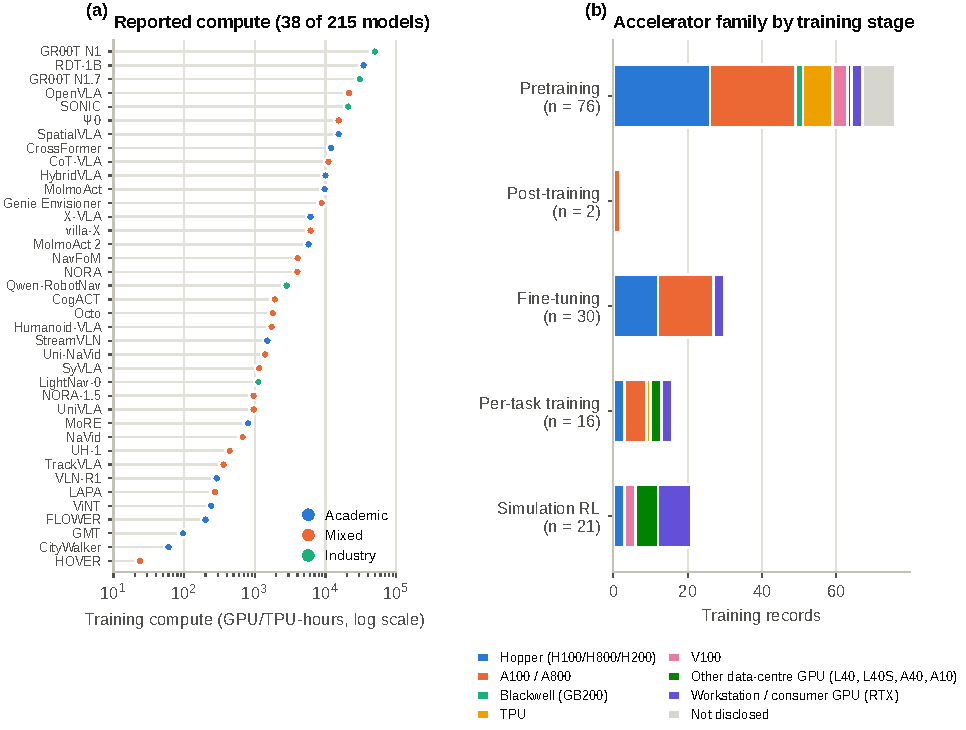
\includegraphics[width=\linewidth]{figures/fig5_training}
\end{adjustwidth}
\caption{Training resources. (\textbf{a}) Pretraining GPU/TPU-hours for the \nGPUh{} models where they are reported or computable, coloured by developer sector. (\textbf{b}) Accelerator family of each training record by stage.\label{fig:training}}
\end{figure}

\subsection{Training Compute}

Only \nGPUh{} models report pretraining compute or both of its factors (Figure~\ref{fig:training}a). Their median is \medGPUh{} GPU/TPU-hours (interquartile range \qOneGPUh--\qThreeGPUh), from \minGPUh{} hours for HOVER~\cite{ax241021229} to roughly \maxGPUh{} H100-hours for GR00T N1~\cite{ax250314734}. Ten models used 10,000 hours or more: besides GR00T N1, these include RDT-1B (about 34,560 H100-hours~\cite{ax241007864}), GR00T N1.7 (30,720 GB200-hours~\cite{web-gr00t-n1-7}) and OpenVLA (21,500 A100-hours~\cite{ax240609246}). Thirteen used fewer than 1,000 hours. Compute is only weakly related to model size ($\rho=\rhoGpuhParams$, $n=\nGpuhParams$) and to release date ($\rho=\rhoGpuhDate$, $n=\nGPUh$), but it rises with the amount of training data among the \nGpuhData{} models that report both ($\rho=\rhoGpuhData$). Data volume and training length, rather than parameter count, appear to set the cost, although these samples are small. These hours mix accelerator generations, from V100 to GB200 and TPU, and are not normalised to a common unit; they are a lower bound on the true cost because they exclude ablations, failed runs, data processing and simulation.

\subsection{Training Data}

Real-robot data appear in 145 models (mostly teleoperation), simulated or synthetic data in 94, human video in 54, web vision--language data in 45 and motion capture in 19 (a model can use several). Data scale is reported for 184 models but in incompatible units---episodes, trajectories, frames, hours---so we parsed hours only. Fifty-four models report hours of data (median 1,522~h). Sixteen report 10,000~h or more, and the largest figures come from 2025--2026 models: 270,000~h of real-world manipulation data for GEN-0~\cite{web-gen-0}, over 500,000~h of data from human wearable devices for GEN-1~\cite{web-gen-1}, and over one million hours of video for DYNA-2 (egocentric human video)~\cite{web-dyna-2} and V-JEPA~2-AC (internet video)~\cite{ax250609985}. Together with studies of data scaling in imitation learning~\cite{ax241018647} and large open datasets such as Open X-Embodiment~\cite{ax231008864} and DROID~\cite{khazatsky2024droid}, these figures indicate that the field is now scaling data faster than parameters.

%%%%%%%%%%%%%%%%%%%%%%%%%%%%%%%%%%%%%%%%%%
\section{Disclosure Audit}\label{sec:disclosure}

Figure~\ref{fig:disclosure} shows the share of models that disclose each of the twelve items. What a model is made of is usually reported: the backbone (87\%), the head type (87\%) and the scale of the training data (86\%). What it costs is not. Training accelerators are named for 47\% of models, training duration for 27\%, pretraining GPU-hours can be computed for 18\% and inference memory is reported for 13\%. Only 41\% report a control rate and 51\% name the inference device. Half (53\%) report a total parameter count, the single number that the memory estimate in Section~\ref{sec:estimator} needs most.

\begin{figure}[H]
\centering
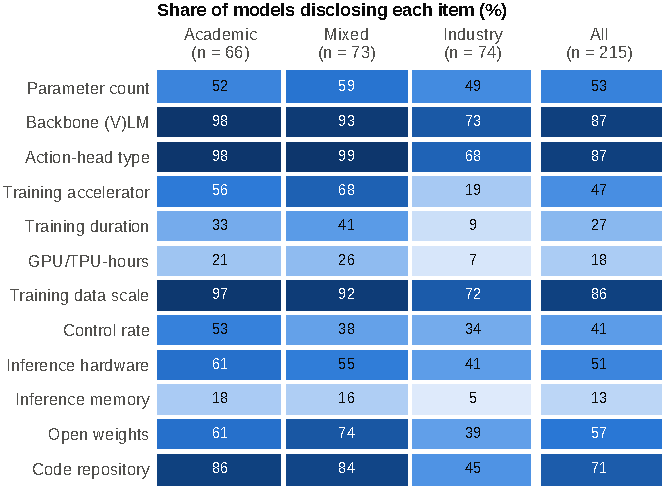
\includegraphics[width=0.82\textwidth]{figures/fig6_disclosure}
\caption{Share of models that disclose each resource item, by developer sector. Two models with unknown affiliation are counted only in ``All''.\label{fig:disclosure}}
\end{figure}

Disclosure differs by sector (Table~\ref{tab:tests}). Industry-only models disclose eight of the twelve items significantly less often than other models after Holm correction. The gaps are widest for training cost: 19\% of industry-only models name a training accelerator against 63\% of the others, 9\% against 37\% report a training duration, and 7\% against 24\% allow GPU-hours to be computed. Industry-only models also disclose the head type less often (68\% against 99\%), release weights less often (39\% against 63\%) and have an official repository less often (45\% against 85\%). The parameter count is the exception: about half of the models in every sector report it. Counting items, the median model discloses 6 of the 12; the medians are 7 for academic-only and mixed teams and 4.5 for industry-only teams.

\begin{table}[H]
\caption{Disclosure of each item by industry-only models versus all other models (academic-only and mixed teams; two models with unknown affiliation excluded). OR: odds ratio from Fisher's exact test; $p_\text{Holm}$: Holm-adjusted $p$-value over the 12 items.\label{tab:tests}}
\small
\begin{tabularx}{\textwidth}{@{}X r r r r@{}}
\toprule
\textbf{Item} & \textbf{Industry (n = 74)} & \textbf{Other (n = 139)} & \textbf{OR} & $\boldsymbol{p}_\textbf{Holm}$\\
\midrule
Parameter count & 36 (49\%) & 77 (55\%) & 0.76 & 0.39\\
Backbone (V)LM & 54 (73\%) & 133 (96\%) & 0.12 & <0.001\\
Action-head type & 50 (68\%) & 137 (99\%) & 0.03 & <0.001\\
Training accelerator & 14 (19\%) & 87 (63\%) & 0.14 & <0.001\\
Training duration & 7 (9\%) & 52 (37\%) & 0.17 & <0.001\\
GPU/TPU-hours & 5 (7\%) & 33 (24\%) & 0.23 & 0.01\\
Training data scale & 53 (72\%) & 131 (94\%) & 0.15 & <0.001\\
Control rate & 25 (34\%) & 63 (45\%) & 0.62 & 0.22\\
Inference hardware & 30 (41\%) & 80 (58\%) & 0.50 & 0.07\\
Inference memory & 4 (5\%) & 24 (17\%) & 0.27 & 0.07\\
Open weights & 29 (39\%) & 88 (63\%) & 0.37 & 0.005\\
Code repository & 33 (45\%) & 118 (85\%) & 0.14 & <0.001\\
\bottomrule
\end{tabularx}
\end{table}


Disclosure is also falling over time. Between 2024 and 2026, the share of models that name a training accelerator fell from 57\% to 31\%, that report a training duration from 37\% to 12\% and that disclose the head type from 97\% to 67\%. Part of the 2026 drop may be temporary, because some 2026 releases have so far been described only in blog posts that may be followed by papers; but the gap between sectors is present in every year. The practical consequence is a selection bias: any comparison of training cost or inference speed across VLAs is, in effect, a comparison among academic and open models.

%%%%%%%%%%%%%%%%%%%%%%%%%%%%%%%%%%%%%%%%%%
\section{Estimating Deployment Feasibility}\label{sec:estimator}

The disclosure audit shows that latency and memory are rarely reported for the device a reader cares about. We therefore estimate them from the few quantities that are usually available---total parameters, head type, chunk structure---and from device specifications, and we test the estimate against every published latency measurement in the corpus.

\subsection{Memory}

The inference memory of a model with $P$ billion parameters stored at $b$ bytes per parameter is estimated as
\begin{equation}
M = P\,b + 1~\text{GB} + 0.3~\text{GB} \times P, \label{eq:mem}
\end{equation}
where the constant term covers the runtime and the last term activations, key--value caches and the vision encoder's working memory. A model is taken to fit when $M$ is at most 90\% of device memory, or 75\% on Jetson modules, whose memory is shared with the CPU. Quantised precisions ($b=1$ for int8 and $b=0.5$ for int4) assume that a working quantised implementation exists, as for NaVILA with AWQ~\cite{ax241204453,lin2024awq}.

\subsection{Latency}

Each network pass is modelled with a roofline~\cite{williams2009roofline}: it takes as long as the slower of reading the weights from memory and doing the arithmetic, plus a fixed overhead. For a network of $p$ billion parameters processing $n$ tokens on a device with memory bandwidth $B_\text{mem}$ (GB/s) and dense BF16 throughput $F_\text{bf16}$ (TFLOPS),
\begin{equation}
f(p, n) = \max\!\left(\frac{1000\,p\,b}{\beta B_\text{mem}},\; \frac{2\,p\,n}{\varphi F_\text{bf16}}\right) + c_0 \quad [\text{ms}], \label{eq:pass}
\end{equation}
where $\beta$ and $\varphi$ are the achievable fractions of peak bandwidth and compute and $c_0$ is a per-pass overhead. The latency of one inference, which produces one action or one action chunk, depends on the head:
\begin{align}
L_\text{tokens} &= f(P, n_\text{in}) + n_\text{tok}\left(\frac{1000\,P\,b}{\beta B_\text{mem}} + c_t\right), \label{eq:ar}\\
L_\text{iterative} &= f(P - P_h, n_\text{in}) + K f(P_h, 50), \label{eq:iter}\\
L_\text{single} &= f(P, n_\text{in}). \label{eq:single}
\end{align}
Token heads (Equation~\eqref{eq:ar}) run one prefill pass over $n_\text{in}$ input tokens and then decode $n_\text{tok}$ action tokens, each of which re-reads the weights; this is the memory-bound regime of autoregressive decoding~\cite{pope2023inference}. Flow-matching and diffusion heads (Equation~\eqref{eq:iter}) run the backbone once and a head of $P_h$ parameters $K$ times over about 50 action tokens. Regression, CVAE and RL heads (Equation~\eqref{eq:single}) need one pass. On Jetson modules the result is multiplied by $\gamma$ to account for lower sustained clocks and less mature kernels. The defaults are $n_\text{in}=600$ input tokens for models with a VLM (1,500 for navigation models that encode video history) and 64 otherwise, $n_\text{tok}=7$ (5 for navigation) unless the source states the number of tokens per action, $K=10$ unless the source states the number of steps. When the head size is not reported, $P_h$ is set to 0.3B for VLM-based models of at least 1.5B parameters, to $0.25P$ for smaller VLM-based models and to $0.7P$ for models without a VLM, whose head is most of the network. Token policies without a language model, such as RT-1~\cite{ax221206817}, emit all action tokens in one pass and are treated as single-pass. Video world-action models are not estimated because their cost depends on the video resolution and horizon.

The estimate needs a total parameter count. When only the language-model size $P_\text{LM}$ is known, we use $P \approx 1.15\,P_\text{LM}$, plus $P_h$ for iterative heads. This is possible for \nEst{} of the \nModels{} models (105 from the total count, 23 from the language-model size); the remaining 87 cannot be assessed.

\subsection{Calibration and Validation}

The corpus contains \nAnchors{} published latency measurements (``anchors'') for \nAnchorModels{} models on \nAnchorDevices{} devices (Table~\ref{tab:anchors} in Appendix~\ref{app:estimator}); 37 can be estimated, the exception being a video world-action model. Device specifications for 24 devices, from the 8~GB Jetson Orin Nano to data-centre GPUs, are listed in Table~\ref{tab:devices}. The five constants were fitted to these anchors and rounded to $\beta=\varphi=0.6$, $c_0=c_t=4$~ms and $\gamma=1.5$; a finer grid search reaches a median error of \refitMed$\times$ on the same anchors, so rounding costs little. Accuracy is measured as the fold error $\max(\hat L/L, L/\hat L)$.

\begin{figure}[H]
\begin{adjustwidth}{-\extralength}{0cm}
\centering
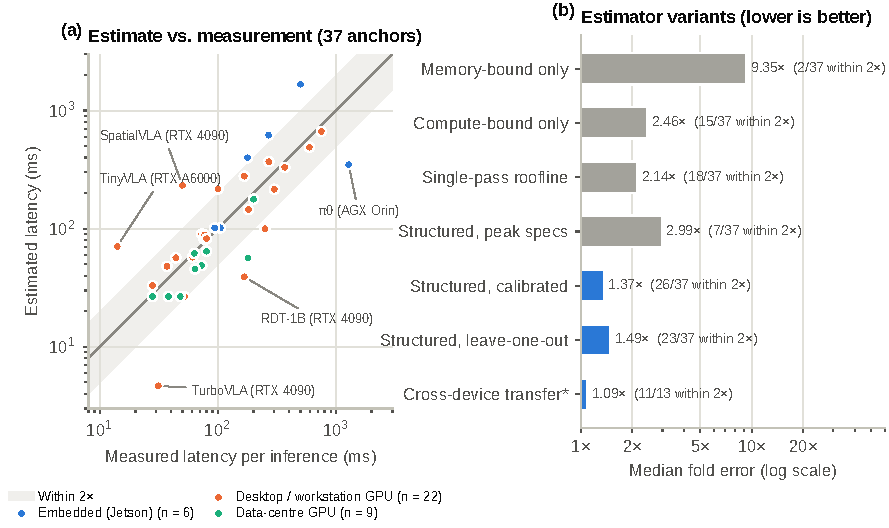
\includegraphics[width=\linewidth]{figures/fig7_estimator}
\end{adjustwidth}
\caption{Validation of the latency estimator. (\textbf{a}) Estimated against measured latency for the 37 anchors; the shaded band marks agreement within a factor of two, and the five largest errors are labelled. (\textbf{b}) Median fold error of estimator variants. *Cross-device transfer predicts each anchor from another measurement of the same model ($n=13$).\label{fig:estimator}}
\end{figure}

With the calibrated constants the median fold error is \calMed$\times$, and \calWithinTwo{} of the 37 anchors are within a factor of two (\calWithinOneFive{} within 1.5$\times$; Figure~\ref{fig:estimator}, Table~\ref{tab:variants}). The estimate is nearly unbiased: the geometric mean of the estimated-to-measured ratio is \calBias. Because the constants were fitted to the same anchors, we also ran a leave-one-out test, refitting the constants on 36 anchors and predicting the held-out one. The out-of-sample median error is \looMed$\times$ with \looWithinTwo{} of 37 within a factor of two, so the in-sample figure is only mildly optimistic.

\begin{table}[H]
\caption{Accuracy of estimator variants on the published latency anchors. Fold error is $\max(\hat L/L, L/\hat L)$; bias is the geometric mean of $\hat L/L$ (values below 1 mean underestimation). The first three variants use the calibrated efficiency constants; ``peak specifications'' uses $\beta=\varphi=\gamma=1$ and no fixed overheads.\label{tab:variants}}
\small
\begin{tabularx}{\textwidth}{@{}X r r r r r@{}}
\toprule
\textbf{Variant} & \textbf{n} & \textbf{Median fold error} & \textbf{$\le$1.5$\times$} & \textbf{$\le$2$\times$} & \textbf{Bias}\\
\midrule
Memory-bound only (weights read once) & 37 & 9.35$\times$ & 0 & 2 & 0.09\\
Compute-bound only ($2Pn$ FLOPs) & 37 & 2.46$\times$ & 8 & 15 & 0.26\\
Single-pass roofline, no head structure & 37 & 2.14$\times$ & 10 & 18 & 0.39\\
Structured roofline, peak specifications & 37 & 2.99$\times$ & 7 & 7 & 0.28\\
Structured roofline, calibrated (this work) & 37 & 1.37$\times$ & 23 & 26 & 0.95\\
Structured roofline, leave-one-out & 37 & 1.49$\times$ & 19 & 23 & 0.87\\
Transfer from another measurement of the same model & 13 & 1.09$\times$ & 10 & 11 & 0.93\\
\bottomrule
\end{tabularx}
\end{table}


Each part of the model earns its place. Using peak specifications without calibration underestimates latency by a factor of about 3.6 (median error \nomMed$\times$, \nomWithinTwo{} of 37 within 2$\times$). With calibrated constants, a memory-bound-only model (weights read once) errs by a median of 9.35$\times$, a compute-bound-only model by 2.46$\times$ and a single-pass roofline that ignores the head structure by 2.14$\times$. Representing token decoding and iterative denoising explicitly is what brings the error down to \calMed$\times$. This supports the qualitative claim of Grover et al.~\cite{grover2026edge} that autoregressive VLAs are bandwidth-bound and diffusion-style heads compute-bound, and puts numbers on it.

Errors are smallest on desktop and data-centre GPUs (median 1.30$\times$ on 19 desktop anchors and 1.40$\times$ on 9 data-centre anchors) and largest on Jetson modules (2.28$\times$ on 6 anchors), where power modes, unified memory and software maturity vary most. The five largest errors fall into three groups. For very small models such as TurboVLA (0.2B)~\cite{ax260727205}, fixed software overheads dominate and the estimate understates latency 6.7-fold. For TinyVLA~\cite{ax240912514} and SpatialVLA~\cite{ax250115830}, the head structure or the number of decoded tokens that we had to assume overstates the work, and the estimate overstates latency about fivefold. For RDT-1B~\cite{ax241007864} and for $\pi_0$ on a Jetson AGX Orin~\cite{ax241024164}, the measurement probably includes work that the estimate does not model, such as separate text or image encoders, preprocessing or a slower power mode, and the estimate understates latency about fourfold.

When a model has been measured on one device, the estimator can transfer that measurement to another device by scaling it with the ratio of the two estimates. On the 13 anchors that have a second anchor of the same model, this transfer has a median error of only \trMed$\times$, with \trWithinTwo{} of 13 within a factor of two. The gallery therefore uses a measured value when one exists for the same device and precision, a transferred value when the model was measured on another device, and the pure estimate otherwise.

\subsection{Which Models Run Where}

Figure~\ref{fig:deploy} applies the estimator to the 126 models that can be assessed on eleven representative devices. A model counts as deployable if it fits in memory and the estimated rate, or the measured or transferred rate when available, is at least 10~Hz. Three regimes appear. On 8--16~GB Jetson modules memory is the binding constraint: in bf16, 89 of the 126 models do not fit in the 8~GB of an Orin Nano and 54 do not fit in the 16~GB of an Orin NX, and only 19 and 20 models reach 10~Hz. On the 64~GB AGX Orin almost everything fits (six models do not) but most models are too slow: 24 reach 10~Hz and 95 run but below 10~Hz. On desktop and data-centre GPUs both constraints relax, and 68 models reach 10~Hz on an RTX 4090, 78 on an RTX 5090 and 105 on an H100.

\begin{figure}[H]
\begin{adjustwidth}{-\extralength}{0cm}
\centering
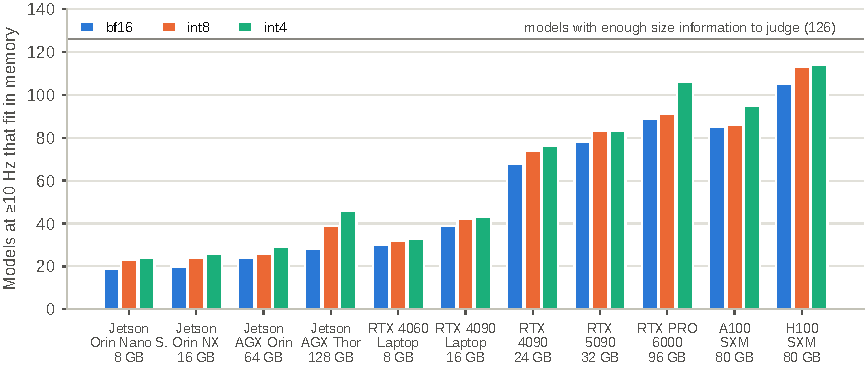
\includegraphics[width=\linewidth]{figures/fig8_deploy}
\end{adjustwidth}
\caption{Number of models estimated to fit in memory and run at 10~Hz or faster on eleven devices, by inference precision. The horizontal line marks the 126 models with enough size information to be assessed.\label{fig:deploy}}
\end{figure}

Quantisation helps most where decoding dominates. On the Jetson AGX Thor, moving from bf16 to int4 raises the number of models at 10~Hz from 28 to 46, and at 5~Hz from 66 to 84, because token-decoding models become faster when fewer bytes are read. On the Orin Nano, int4 lets 45 more models fit in memory, but most of them are too slow, so the number at 10~Hz rises only from 19 to 24. The largest models that reach 10~Hz on an Orin Nano in bf16 are TinyVLA (1.3B)~\cite{ax240912514} and HPT (1.1B)~\cite{ax240920537}; on an RTX 4090 they include 7B models such as TrackVLA~\cite{ax250523189} and 5B models such as $\pi_{0.7}$~\cite{ax260415483}. These are estimates for batch size one without compiler or kernel optimisation; optimised runtimes such as TensorRT, which GR00T N1.7 uses for its reported latencies~\cite{web-gr00t-n1-7}, can change measured rates substantially.

\subsection{Fine-Tuning Cost}

A similar estimate covers fine-tuning. Per-GPU memory is the sum of model state and activations. Full fine-tuning with mixed-precision Adam needs about 16 bytes per parameter (bf16 weights and gradients, an fp32 master copy and two optimiser moments~\cite{rajbhandari2020zero}), divided by the number of GPUs when the state is sharded~\cite{rajbhandari2020zero,zhao2023fsdp}. LoRA~\cite{hu2021lora} keeps frozen bf16 weights (2~bytes per parameter) and trains adapters with 1\% of the parameters; QLoRA~\cite{dettmers2023qlora} stores the frozen weights in 4~bits (about 0.55~bytes per parameter); training only the action head keeps the backbone frozen in bf16. Activations are modelled as 2~GB plus 1.5~GB per billion parameters for small batches and 4~GB plus 5~GB per billion for typical batches. These activation constants were set to match three reported requirements---more than 22.5~GB for LoRA and more than 70~GB for full fine-tuning of $\pi_0$, about 27~GB for LoRA on OpenVLA at batch size one, and about 70~GB for full fine-tuning of GO-1~\cite{ax241024164,ax240609246,ax250306669}---and, unlike the latency model, have not been validated on independent measurements. Training time follows the usual $6PN$ rule~\cite{kaplan2020scaling} ($4PN$ for adapter training, $2PN$ for a frozen backbone) at 35\% of peak BF16 throughput and 90\% scaling efficiency across GPUs.

\begin{table}[H]
\caption{Estimated fine-tuning feasibility for the 89 models with released weights and enough size information. Each cell gives the number of models whose estimated per-GPU memory fits (90\% of device memory; 75\% on Jetson) and, in parentheses, the largest such model (total parameters). Memory assumes the ``normal'' activation budget (4~GB + 5~GB per billion parameters per GPU). Head-only applies to models with a separable flow-matching, diffusion or hybrid head; where the source does not give the head size, the estimator's default is used.\label{tab:tune}}
\small
\begin{tabularx}{\textwidth}{@{}X c c c c@{}}
\toprule
\textbf{Configuration} & \textbf{Full} & \textbf{LoRA} & \textbf{QLoRA} & \textbf{Head only}\\
\midrule
1$\times$ RTX 4090 (24 GB) & 20 ($\le$0.77B) & 32 ($\le$2.37B) & 46 ($\le$3B) & 34 ($\le$5.1B)\\
1$\times$ RTX 5090 (32 GB) & 26 ($\le$1.1B) & 48 ($\le$3.3B) & 56 ($\le$4.2B) & 39 ($\le$7.6B)\\
1$\times$ A100 (80 GB) & 47 ($\le$3.2B) & 86 ($\le$9B) & 86 ($\le$9B) & 44 ($\le$8.45B)\\
8$\times$ H100 (80 GB) & 86 ($\le$9B) & 86 ($\le$9B) & 86 ($\le$9B) & 44 ($\le$8.45B)\\
Jetson AGX Thor (128 GB) & 56 ($\le$4.2B) & 86 ($\le$9B) & 88 ($\le$14B) & 44 ($\le$8.45B)\\
\bottomrule
\end{tabularx}
\end{table}


Table~\ref{tab:tune} shows what this implies for the 86 open-weight models that can be assessed. A single 24~GB RTX 4090 can fully fine-tune only models below about 0.8B parameters (19 models), but LoRA reaches 2.4B (30 models) and QLoRA 3B (44 models). One 80~GB A100 is enough for LoRA on 83 of the 86 models, up to 9B; the remaining three are the largest in the set (two 14B models and a system whose planner is a 72B VLM). For example, the estimate for LoRA on OpenVLA (7B) is about 54~GB at a typical batch size, so it needs an 80~GB GPU, and 10,000 steps at a global batch of 32 take an estimated 14~h on one A100; on eight H100 GPUs, full fine-tuning of $\pi_0$ takes an estimated 23~min.

%%%%%%%%%%%%%%%%%%%%%%%%%%%%%%%%%%%%%%%%%%
\section{Reinforcement Learning in VLA Pipelines}\label{sec:rl}

Most models in the corpus are trained by imitation alone: \nRLnone{} do not use RL, \nRLuse{} use it as a core component, \nRLpart{} use it partially and \nRLund{} do not say. Where RL appears, it enters at one of six points, and the point depends strongly on the domain (Figure~\ref{fig:rlbase}a). In humanoid models RL trains the controller: 13 humanoid models are RL-trained whole-body controllers, often motion trackers learned in simulation~\cite{ax241021229,ax250808241,ax251107820}, and 12 place an RL low-level controller under a VLA that issues commands or latent goals~\cite{ax250613751}. Mobile manipulation follows the same pattern on legged robots, with RL-trained controllers in five models and RL low-level controllers in four~\cite{ax240316967,ax240317367}.

\begin{figure}[H]
\begin{adjustwidth}{-\extralength}{0cm}
\centering
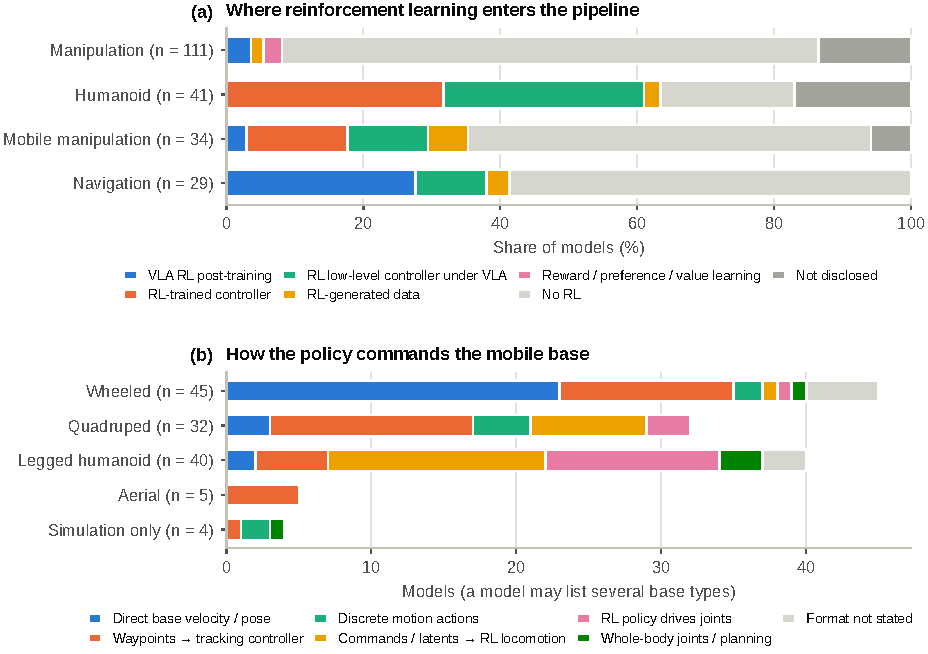
\includegraphics[width=0.86\linewidth]{figures/fig9_rl_base}
\end{adjustwidth}
\caption{(\textbf{a}) Where reinforcement learning enters the pipeline, by domain. (\textbf{b}) How the policy commands the mobile base, by base type; a model can list more than one base type.\label{fig:rlbase}}
\end{figure}

RL post-training of the VLA itself is the newest use and is concentrated in navigation. Of the 13 models that fine-tune the VLA with RL, eight are navigation models~\cite{ax250216372,ax241214401,ax250617221,ax260211598,ax260108665,ax260202459,ax260830935,ax260530280}. They train in simulation, where rewards such as progress towards a goal are cheap to compute, using PPO-style objectives~\cite{schulman2017ppo} or group-relative policy optimisation (GRPO)~\cite{shao2024deepseekmath}. In manipulation, RL post-training is rarer (four models) and relies on real-robot or offline data: $\pi^*_{0.6}$ learns a value function from demonstrations, autonomous rollouts and human corrections and uses it to improve the policy~\cite{ax251114759}, GR-RL runs online RL on a real robot~\cite{ax251201801}, and SyVLA optimises the whole VLA with a PPO variant on a real robot~\cite{ax260609009}. One quadruped model applies offline RL to its VLA~\cite{ax250308007}. Three manipulation models use reward, preference or value learning without full RL post-training, and six models across domains use data generated by RL policies. Because simulation RL runs on one or a few GPUs (Section~\ref{sec:training}), adding an RL controller changes the training budget far less than VLA pretraining does.

%%%%%%%%%%%%%%%%%%%%%%%%%%%%%%%%%%%%%%%%%%
\section{Commanding the Mobile Base}\label{sec:base}

\nMobile{} models control a robot with a mobile base: 45 wheeled, 32 quadruped, 40 legged humanoid, five aerial and four simulation-only platforms (a model can list several). How the policy talks to the base is rarely stated in one place, so we coded it into eight classes (Figure~\ref{fig:rlbase}b). The interface follows the platform. On wheeled robots the policy usually outputs base velocities or poses directly (23 models), as RT-1 does~\cite{ax221206817}, or waypoints for a tracking controller (12), as in the navigation foundation models GNM, ViNT and NoMaD~\cite{ax221003370,ax230614846,ax231007896}. On quadrupeds waypoints dominate (14 models), followed by commands or latents for an RL locomotion controller (8). On humanoids the policy almost never drives the base directly: 15 models send commands or latent goals to an RL locomotion controller and 12 are themselves RL policies that drive the joints. All five aerial models output waypoints. Eight models do not state the interface at all.

These choices matter for resources. A policy that outputs waypoints or latent commands can run at a few hertz while a separately trained controller closes the loop at hundreds of hertz, which is how large VLMs are used on legged robots despite the latencies in Section~\ref{sec:estimator}. The cost is that the controller, its training and its rate become part of the system that must be reported.

%%%%%%%%%%%%%%%%%%%%%%%%%%%%%%%%%%%%%%%%%%
\section{Discussion}\label{sec:discussion}

\subsection{Implications for Practitioners}

Three practical lessons follow. First, check memory before speed on small embedded computers and speed before memory on large ones. Most of the assessable models do not fit in bf16 on an 8~GB Orin Nano and almost half do not fit on a 16~GB Orin NX, so quantisation is the first lever there; on 64--128~GB modules nearly everything fits, and the head structure and chunking decide whether the policy is fast enough. Second, the head structure matters as much as the parameter count. A 3B model with a flow-matching head and 50-step chunks can control a robot at 50~Hz on a desktop GPU~\cite{ax241024164}, whereas a 7B model that decodes several tokens per action is limited by memory bandwidth to a few hertz~\cite{ax240609246} unless it uses parallel decoding and chunking~\cite{ax250219645}. Third, fine-tuning is within reach of a single workstation for most open models below about 3B parameters if LoRA or QLoRA is used, whereas full fine-tuning of 7B-class models still needs several 80~GB GPUs. The gallery that accompanies this review performs these checks for any of the \nDevices{} devices in Table~\ref{tab:devices} or for user-supplied specifications.

\subsection{A Reporting Checklist}

The disclosure audit points to a small set of numbers that, if reported consistently, would make the estimates above unnecessary. Table~\ref{tab:checklist} lists ten items, in the spirit of model cards~\cite{mitchell2019modelcards}, datasheets~\cite{gebru2021datasheets}, reproducibility checklists~\cite{pineau2021reproducibility} and calls to report compute and energy~\cite{strubell2019,schwartz2020green,henderson2020energy}. Most cost the authors little: they are already known when the paper is written.

\begin{table}[H]
\caption{A ten-item checklist for reporting the resources of robot foundation policies.\label{tab:checklist}}
\small
\begin{tabularx}{\textwidth}{@{}r X X@{}}
\toprule
\textbf{\#} & \textbf{Item} & \textbf{Why it matters}\\
\midrule
1 & Total parameters, split into vision encoder, backbone and action head, with the precision used at inference & Sets memory and the bandwidth-bound part of latency; reported by only 53\% of models\\
2 & Action representation: head type, chunk length, tokens per action or denoising steps & Determines how latency scales with model size (Equations~\eqref{eq:ar}--\eqref{eq:single})\\
3 & For each training stage: accelerator model, count, wall-clock duration, steps and batch size & Allows GPU-hours to be computed; only 18\% of models allow this today\\
4 & Training data by source type (teleoperation, simulation, human video, web), in hours and episodes & Data volume, more than parameter count, tracks training cost (Section~\ref{sec:training})\\
5 & Fine-tuning recipe: method (full, LoRA, head only), GPUs, memory, steps and time & Tells users whether adaptation fits their hardware\\
6 & Inference latency per action chunk on a named device, with precision, batch size and software stack & Enables like-for-like comparison and calibration of estimators\\
7 & Peak inference memory on that device & Reported by only 13\% of models\\
8 & Control rate on the robot and where inference runs (onboard, local PC, remote server), including network latency & Separates model speed from system design\\
9 & Interface to the robot: what the policy outputs, at what rate, and to which low-level controller & Required to reproduce mobile and humanoid systems (Section~\ref{sec:base})\\
10 & Release status of weights, code and training data, with licences, and any RL use with its simulation budget & Determines whether the model can be studied or deployed by others\\
\bottomrule
\end{tabularx}
\end{table}

Standard benchmarks of inference speed for robot policies, analogous to MLPerf for data-centre inference~\cite{reddi2020mlperf}, would complement such reporting. The anchors in Table~\ref{tab:anchors} show the problem: they were measured by different authors with different software stacks and sometimes include image preprocessing or network transfer, which limits how precisely any estimator can be calibrated.

\subsection{Limitations}

The review has several limitations. The corpus is large but not exhaustive; it reflects the search described in Section~\ref{sec:methods} and the reference dates of 6--19 October 2026, and the field moves fast enough that some 2026 models will have published papers after the cut-off. All values are self-reports by the developers; we did not reproduce training runs or measure latencies ourselves, and \nUnverified{} records could not be fully verified. Coding the head family, the RL category, the base interface and the developer sector involves judgement, and inter-rater agreement was not measured. GPU-hours mix accelerator generations and exclude experimentation, so they understate true cost and should not be compared across generations without care.

The estimator is deliberately simple. It assumes batch size one, ignores compiler and kernel optimisation, assumes that quantised kernels exist, and treats a dual-system pipeline as a single network, which can make it optimistic for hierarchical models such as Helix whose large VLM runs at a lower rate than the action module. It needs a parameter count, so 87 models cannot be assessed, and it was validated on only 37 anchors, six of them on embedded devices. The fine-tuning estimates rest on three reported memory requirements and have not been validated independently. The estimates should therefore be read as screening tools, accurate to within a factor of two for about two thirds of the anchors, not as substitutes for measurement.

\subsection{Future Work}

Three extensions would strengthen this line of work: a shared protocol and open harness for measuring VLA latency, memory and energy on common devices, which would multiply the number and quality of anchors; adding energy and power to the coded resources, which matters for battery-powered robots; and keeping the dataset current, which the open gallery and scripts make possible.

%%%%%%%%%%%%%%%%%%%%%%%%%%%%%%%%%%%%%%%%%%
\section{Conclusions}\label{sec:conclusions}

We reviewed \nModels{} robot policy models from October 2022 to October 2026 from the perspective of the resources they need to be trained and deployed. The architecture has moved towards flow-matching heads, action chunking and Qwen-family backbones of about 2--8B parameters, and model size has plateaued at a median of about 4B parameters since 2025, while training data have grown to hundreds of thousands of hours. Training cost spans more than three orders of magnitude, from tens to tens of thousands of GPU-hours, but it is reported for fewer than one model in five, and industry-only models disclose training hardware, training duration and compute far less often than academic and mixed teams. A roofline estimator that represents token decoding and iterative denoising predicts published latencies to a median factor of \calMed{} (\looMed{} out of sample) and shows that memory limits deployment on small embedded computers while speed limits it on larger ones. We hope that the dataset, the estimator and the reporting checklist will make resource numbers a routine part of how robot foundation models are described.

\vspace{6pt}

%%%%%%%%%%%%%%%%%%%%%%%%%%%%%%%%%%%%%%%%%%
\authorcontributions{% TODO(author): adjust to the actual contributions (CRediT taxonomy).
Conceptualization, F.L.; methodology, F.L.; software, F.L.; validation, F.L.; formal analysis, F.L.; investigation, F.L.; data curation, F.L.; writing---original draft preparation, F.L.; writing---review and editing, F.L.; visualization, F.L. The author has read and agreed to the published version of the manuscript.}

\funding{This research received no external funding. % TODO(author): confirm, and state who funds the APC.
}

\institutionalreview{Not applicable.}

\informedconsent{Not applicable.}

\dataavailability{The dataset (\nModels{} model records, training-hardware records, device specifications and latency anchors), the analysis scripts that produce every number and figure in this article, and an interactive gallery are openly available at \url{https://github.com/yc424k/vla-gallery} and \url{https://vla-gallery.is-a.dev/}. % TODO(author): make sure the repository is public and add a Zenodo DOI for the archived release.
}

\acknowledgments{During the preparation of this manuscript, the author used Claude (Anthropic) [TODO(author): version] for the purposes of writing analysis and plotting code and drafting the manuscript text [TODO(author): and, if applicable, assisting data extraction and verification]. The author has reviewed and edited the output and takes full responsibility for the content of this publication.}

\conflictsofinterest{The author declares no conflicts of interest.}

%%%%%%%%%%%%%%%%%%%%%%%%%%%%%%%%%%%%%%%%%%
\abbreviations{Abbreviations}{
The following abbreviations are used in this manuscript:
\\

\noindent
\begin{tabular}{@{}ll}
BF16 & Brain floating point, 16 bits\\
CVAE & Conditional variational autoencoder\\
FSDP & Fully sharded data parallel\\
GPU & Graphics processing unit\\
GRPO & Group relative policy optimisation\\
LLM & Large language model\\
LM & Language model\\
LoRA & Low-rank adaptation\\
QLoRA & Quantised low-rank adaptation\\
RL & Reinforcement learning\\
TPU & Tensor processing unit\\
VA & Vision--action (visuomotor policy without a pretrained VLM)\\
VLA & Vision--language--action\\
VLM & Vision--language model\\
\end{tabular}
}

%%%%%%%%%%%%%%%%%%%%%%%%%%%%%%%%%%%%%%%%%%
\appendixtitles{yes}
\appendixstart
\appendix
\section[\appendixname~\thesection]{The Corpus}\label{app:corpus}

Table~\ref{tab:models} lists every model with its key attributes and primary source. Full records, including the source of every value, are in the released dataset.

{\scriptsize
\setlength{\tabcolsep}{3pt}
\begin{longtable}{@{}r p{3.55cm} l l l r l l c r@{}}
\caption{All 215 models in the corpus, ordered by release month. Domain: Manip.\ = manipulation, Hum.\ = humanoid, MoMa = mobile manipulation, Nav.\ = navigation. Params: total parameters in billions (n/d = not disclosed). LM: language-model family of the backbone. Head: action-head family. W: weights released (Y = yes, P = partially, N = no, ? = unverified). GPU-h: pretraining GPU/TPU-hours where both accelerator count and duration are reported.\label{tab:models}}\\
\toprule
\textbf{\#} & \textbf{Model} & \textbf{Date} & \textbf{Domain} & \textbf{Type} & \textbf{Params} & \textbf{LM} & \textbf{Head} & \textbf{W} & \textbf{GPU-h}\\
\midrule
\endfirsthead
\toprule
\textbf{\#} & \textbf{Model} & \textbf{Date} & \textbf{Domain} & \textbf{Type} & \textbf{Params} & \textbf{LM} & \textbf{Head} & \textbf{W} & \textbf{GPU-h}\\
\midrule
\endhead
\bottomrule
\endfoot
1 & GNM~\cite{ax221003370} & 2022-10 & Nav. & VA & 0.0087 & none & regression & Y & \\
2 & RT-1~\cite{ax221206817} & 2022-12 & MoMa & VA & 0.035 & none & tokens & Y & \\
3 & Diffusion Policy (CNN)~\cite{ax230304137} & 2023-03 & Manip. & VA & 0.309 & none & diffusion & Y & \\
4 & Diffusion Policy (Transformer)~\cite{ax230304137} & 2023-03 & Manip. & VA & 0.102 & none & diffusion & Y & \\
5 & ACT~\cite{ax230413705} & 2023-04 & Manip. & VA & 0.08 & none & CVAE & N & \\
6 & ViNT~\cite{ax230614846} & 2023-06 & Nav. & VA & 0.031 & none & regression & Y & 240\\
7 & RT-2~\cite{ax230715818} & 2023-07 & MoMa & VLA & 55 & PaLI/PaLM & tokens & N & \\
8 & NoMaD~\cite{ax231007896} & 2023-10 & Nav. & VA & 0.019 & none & diffusion & Y & \\
9 & RT-1-X~\cite{ax231008864} & 2023-10 & Manip. & VA & 0.035 & none & tokens & Y & \\
10 & RT-2-X~\cite{ax231008864} & 2023-10 & Manip. & VLA & 55 & PaLI/PaLM & tokens & N & \\
11 & RoboFlamingo~\cite{ax231101378} & 2023-11 & Manip. & VLA & 9 & other & regression & Y & \\
12 & GR-1~\cite{ax231213139} & 2023-12 & Manip. & VLA & 0.195 & none & regression & P & \\
13 & HarmonicMM~\cite{ax231206639} & 2023-12 & MoMa & VA & n/d & none & RL policy & N & \\
14 & Octo~\cite{ax240512213} & 2023-12 & Manip. & VA & 0.093 & none & diffusion & Y & 1,792\\
15 & QUAR-VLA (QUART)~\cite{ax231214457} & 2023-12 & MoMa & VLA & 8 & other & tokens & N & \\
16 & SARA-RT~\cite{ax231201990} & 2023-12 & Manip. & Other & n/d & PaLI/PaLM & tokens & N & \\
17 & AutoRT~\cite{ax240112963} & 2024-01 & MoMa & Other & n/d & n/d & other & N & \\
18 & Mobile ALOHA~\cite{ax240102117} & 2024-01 & MoMa & VA & n/d & none & CVAE & N & \\
19 & Humanoid Next-Token Locomotion~\cite{ax240219469} & 2024-02 & Hum. & VA & 0.008 & none & regression & ? & \\
20 & NaVid~\cite{ax240215852} & 2024-02 & Nav. & VLA & 7 & Llama & tokens & Y & 672\\
21 & UMI~\cite{ax240210329} & 2024-02 & Manip. & VA & n/d & none & diffusion & P & \\
22 & 3D-VLA~\cite{ax240309631} & 2024-03 & Manip. & VLA & n/d & other & tokens & P & \\
23 & DP3~\cite{ax240303954} & 2024-03 & Manip. & VA & n/d & none & diffusion & N & \\
24 & Visual Quadrupedal Loco-Manipulation~\cite{ax240320328} & 2024-03 & MoMa & VA & n/d & none & diffusion & N & \\
25 & RFM-1~\cite{web-rfm-1} & 2024-03 & Manip. & VLA & 8 & n/d & n/d & N & \\
26 & RoboDuet~\cite{ax240317367} & 2024-03 & MoMa & Other & n/d & none & RL policy & N & \\
27 & RT-H~\cite{ax240301823} & 2024-03 & MoMa & VLA & 55 & PaLI/PaLM & tokens & N & \\
28 & VBC~\cite{ax240316967} & 2024-03 & MoMa & VA & n/d & none & RL policy & P & \\
29 & VQ-BeT~\cite{ax240303181} & 2024-03 & Manip. & VA & n/d & none & tokens & P & \\
30 & RISE~\cite{ax240412281} & 2024-04 & Manip. & VA & n/d & none & diffusion & N & \\
31 & Tesla Optimus~\cite{web-tesla-optimus} & 2024-05 & Hum. & Other & n/d & n/d & n/d & N & \\
32 & BAKU~\cite{ax240607539} & 2024-06 & Manip. & VA & 0.114 & none & regression & N & \\
33 & HumanPlus HIT~\cite{ax240610454} & 2024-06 & Hum. & VA & n/d & none & regression & ? & \\
34 & HumanPlus HST~\cite{ax240610454} & 2024-06 & Hum. & VA & n/d & none & RL policy & ? & \\
35 & LLaRA~\cite{ax240620095} & 2024-06 & Manip. & VLA & 7 & Llama & tokens & Y & \\
36 & OmniH2O~\cite{ax240608858} & 2024-06 & Hum. & VA & n/d & none & RL policy & ? & \\
37 & OpenVLA~\cite{ax240609246} & 2024-06 & Manip. & VLA & 7 & Llama & tokens & Y & 21,500\\
38 & RoboMamba~\cite{ax240604339} & 2024-06 & Manip. & VLA & 2.8 & Mamba & regression & ? & \\
39 & ECoT~\cite{ax240708693} & 2024-07 & Manip. & VLA & 7 & Llama & tokens & Y & \\
40 & Mobility VLA~\cite{ax240707775} & 2024-07 & Nav. & VLA & n/d & Gemini & other & N & \\
41 & UMI on Legs~\cite{ax240710353} & 2024-07 & MoMa & VA & n/d & none & diffusion & P & \\
42 & CrossFormer~\cite{ax240811812} & 2024-08 & Nav. & VLA & 0.13 & none & regression & Y & 12,032\\
43 & Helpful DoggyBot~\cite{ax241000231} & 2024-09 & MoMa & Other & n/d & none & RL policy & N & \\
44 & HPT~\cite{ax240920537} & 2024-09 & Manip. & VA & 1.1 & none & regression & P & \\
45 & InterACT~\cite{ax240907914} & 2024-09 & Manip. & VA & n/d & none & regression & ? & \\
46 & Robot Utility Models (RUM)~\cite{ax240905865} & 2024-09 & MoMa & VA & n/d & none & tokens & Y & \\
47 & ScaleDP~\cite{ax240914411} & 2024-09 & Manip. & VA & 1 & none & diffusion & ? & \\
48 & TinyVLA~\cite{ax240912514} & 2024-09 & Manip. & VLA & 1.3 & other & diffusion & P & \\
49 & ALOHA Unleashed~\cite{ax241013126} & 2024-10 & Manip. & VA & 0.217 & none & diffusion & ? & \\
50 & Challenging-Terrain Transformer~\cite{ax241003654} & 2024-10 & Hum. & VA & 0.0014 & none & RL policy & ? & \\
51 & Data Scaling Laws~\cite{ax241018647} & 2024-10 & Manip. & VA & 0.396 & none & diffusion & Y & \\
52 & Dita~\cite{ax250319757} & 2024-10 & Manip. & VLA & 0.334 & none & diffusion & Y & \\
53 & EgoMimic~\cite{ax241024221} & 2024-10 & Manip. & VA & n/d & none & regression & ? & \\
54 & GR-2~\cite{ax241006158} & 2024-10 & Manip. & VLA & 0.23 & none & CVAE & ? & \\
55 & HOVER~\cite{ax241021229} & 2024-10 & Hum. & VA & n/d & none & RL policy & ? & 24\\
56 & iDP3~\cite{ax241010803} & 2024-10 & Hum. & VA & n/d & none & diffusion & Y & \\
57 & LAPA~\cite{ax241011758} & 2024-10 & Manip. & VLA & 7 & Llama & latent & Y & 272\\
58 & LeLaN~\cite{ax241003603} & 2024-10 & Nav. & VLA & n/d & none & regression & Y & \\
59 & RDT-1B~\cite{ax241007864} & 2024-10 & Manip. & VLA & 1.2 & none & diffusion & Y & 34,560\\
60 & X-Mobility~\cite{ax241017491} & 2024-10 & Nav. & VA & n/d & none & regression & Y & \\
61 & $\pi_0$~\cite{ax241024164} & 2024-10 & Manip. & VLA & 3.3 & Gemma & flow & Y & \\
62 & CityWalker~\cite{ax241117820} & 2024-11 & Nav. & VA & 0.214 & none & regression & Y & 60\\
63 & CogACT~\cite{ax241119650} & 2024-11 & Manip. & VLA & 7.6 & Llama & diffusion & Y & 1,920\\
64 & TidyBot++ (diffusion policy)~\cite{ax241210447} & 2024-11 & MoMa & VA & n/d & none & diffusion & P & \\
65 & CARP~\cite{ax241206782} & 2024-12 & Manip. & VA & 0.0161 & none & tokens & Y & \\
66 & DiVLA (Diffusion-VLA)~\cite{ax241203293} & 2024-12 & Manip. & VLA & 72 & Qwen & diffusion & ? & \\
67 & ExBody2~\cite{ax241213196} & 2024-12 & Hum. & VA & n/d & none & RL policy & ? & \\
68 & MiniVLA~\cite{web-minivla} & 2024-12 & Manip. & VLA & 1 & Qwen & tokens & Y & \\
69 & Moto~\cite{ax241204445} & 2024-12 & Manip. & VA & 0.098 & none & latent & Y & \\
70 & NaVILA~\cite{ax241204453} & 2024-12 & Nav. & VLA & 8 & Llama & tokens & Y & \\
71 & NWM (Navigation World Models)~\cite{ax241203572} & 2024-12 & Nav. & Other & 1 & none & video WM & Y & \\
72 & QUART-Online~\cite{ax241215576} & 2024-12 & MoMa & VLA & 8 & other & tokens & Y & \\
73 & RING (The One RING)~\cite{ax241214401} & 2024-12 & Nav. & VLA & n/d & none & tokens & Y & \\
74 & TraceVLA~\cite{ax241210345} & 2024-12 & Manip. & VLA & 7 & Llama & tokens & Y & \\
75 & UH-1 (Humanoid-X)~\cite{ax241214172} & 2024-12 & Hum. & Other & n/d & none & tokens & ? & 440\\
76 & Uni-NaVid~\cite{ax241206224} & 2024-12 & Nav. & VLA & 7 & Llama & tokens & Y & 1,400\\
77 & SLIM~\cite{ax250109905} & 2025-01 & MoMa & VLA & 0.019 & none & RL policy & N & \\
78 & SpatialVLA~\cite{ax250115830} & 2025-01 & Manip. & VLA & 3.5 & Gemma & tokens & Y & 15,360\\
79 & $\pi_0$-FAST~\cite{ax250109747} & 2025-01 & Manip. & VLA & 3 & Gemma & tokens & Y & \\
80 & COMPASS~\cite{ax250216372} & 2025-02 & Nav. & VA & n/d & none & RL policy & P & \\
81 & DexGraspVLA~\cite{ax250220900} & 2025-02 & Manip. & VLA & n/d & Qwen & diffusion & Y & \\
82 & DexVLA~\cite{ax250205855} & 2025-02 & Manip. & VLA & n/d & Qwen & diffusion & P & \\
83 & Figure Helix~\cite{web-figure-helix} & 2025-02 & Hum. & VLA & 7.1 & n/d & regression & N & \\
84 & Hi Robot~\cite{ax250219417} & 2025-02 & Manip. & VLA & n/d & Gemma & flow & N & \\
85 & Humanoid-VLA~\cite{ax250214795} & 2025-02 & Hum. & VLA & n/d & Llama & tokens & ? & 1,728\\
86 & Magma~\cite{ax250213130} & 2025-02 & Manip. & VLA & 8.6 & Llama & tokens & Y & \\
87 & OpenVLA-OFT~\cite{ax250219645} & 2025-02 & Manip. & VLA & 7 & Llama & regression & Y & \\
88 & BRS (WB-VIMA)~\cite{ax250305652} & 2025-03 & MoMa & VA & n/d & none & diffusion & ? & \\
89 & CoT-VLA~\cite{ax250322020} & 2025-03 & Manip. & VLA & 7 & Llama & tokens & ? & 11,000\\
90 & Dense Policy~\cite{ax250313217} & 2025-03 & Manip. & VA & n/d & none & regression & N & \\
91 & Figure RL walking controller~\cite{web-figure-rl} & 2025-03 & Hum. & VA & n/d & none & RL policy & N & \\
92 & Gemini Robotics~\cite{ax250320020} & 2025-03 & Manip. & VLA & n/d & Gemini & n/d & N & \\
93 & Gemini Robotics-ER~\cite{ax250320020} & 2025-03 & Manip. & Other & n/d & Gemini & other & N & \\
94 & GO-1 (Genie Operator-1)~\cite{ax250306669} & 2025-03 & MoMa & VLA & 3 & InternLM & diffusion & Y & \\
95 & GR00T N1~\cite{ax250314734} & 2025-03 & Hum. & VLA & 2.2 & SmolLM & flow & Y & 50,000\\
96 & HAT~\cite{ax250313441} & 2025-03 & Hum. & VA & n/d & none & CVAE & ? & \\
97 & HybridVLA~\cite{ax250310631} & 2025-03 & Manip. & VLA & 7 & Llama & hybrid & Y & 10,000\\
98 & MoManipVLA~\cite{ax250313446} & 2025-03 & MoMa & VLA & 7 & Llama & tokens & N & \\
99 & MoRE~\cite{ax250308007} & 2025-03 & MoMa & VLA & 9.8 & other & tokens & N & 800\\
100 & NORA~\cite{ax250419854} & 2025-04 & Manip. & VLA & 3 & Qwen & tokens & Y & 4,000\\
101 & $\pi_{0.5}$~\cite{ax250416054} & 2025-04 & MoMa & VLA & n/d & Gemma & flow & P & \\
102 & AMO~\cite{ax250503738} & 2025-05 & Hum. & VA & n/d & none & RL policy & P & \\
103 & GR00T N1.5~\cite{web-gr00t-n1-5} & 2025-05 & Hum. & VLA & 3 & n/d & flow & Y & \\
104 & GraspVLA~\cite{ax250503233} & 2025-05 & Manip. & VLA & n/d & InternLM & flow & Y & \\
105 & NavDP~\cite{ax250508712} & 2025-05 & Nav. & VA & n/d & none & diffusion & Y & \\
106 & TrackVLA~\cite{ax250523189} & 2025-05 & Nav. & VLA & 7 & Llama & diffusion & N & 360\\
107 & TWIST~\cite{ax250502833} & 2025-05 & Hum. & VA & n/d & none & RL policy & Y & \\
108 & UniVLA (OpenDriveLab)~\cite{ax250506111} & 2025-05 & Manip. & VLA & 7 & Llama & latent & Y & 960\\
109 & $\pi_{0.5}$ + KI~\cite{ax250523705} & 2025-05 & Manip. & VLA & n/d & Gemma & hybrid & P & \\
110 & 1X Redwood AI~\cite{web-1x-redwood-ai} & 2025-06 & Hum. & VLA & 0.16 & none & diffusion & N & \\
111 & BumbleBee~\cite{ax250612779} & 2025-06 & Hum. & VA & n/d & n/d & n/d & ? & \\
112 & Chain-of-Action~\cite{ax250609990} & 2025-06 & Manip. & VA & n/d & none & regression & ? & \\
113 & DYNA-1~\cite{web-dyna-1} & 2025-06 & Manip. & Other & n/d & n/d & n/d & N & \\
114 & Gemini Robotics On-Device~\cite{web-gemini-robotics-on-device} & 2025-06 & Manip. & VLA & n/d & Gemini & n/d & N & \\
115 & GMT (General Motion Tracking)~\cite{ax250614770} & 2025-06 & Hum. & VA & n/d & none & RL policy & Y & 96\\
116 & LeVERB~\cite{ax250613751} & 2025-06 & Hum. & VLA & n/d & none & latent & ? & \\
117 & LeVERB-A (LeVERB System 1)~\cite{ax250613751} & 2025-06 & Hum. & VA & n/d & none & RL policy & ? & \\
118 & Real-Time Chunking (inference-time)~\cite{ax250607339} & 2025-06 & Manip. & Other & n/d & Gemma & flow & N & \\
119 & SmolVLA~\cite{ax250601844} & 2025-06 & Manip. & VLA & 2.2 & SmolLM & flow & Y & \\
120 & UniVLA (BAAI)~\cite{ax250619850} & 2025-06 & Manip. & VLA & 8.5 & other & tokens & Y & \\
121 & V-JEPA 2-AC~\cite{ax250609985} & 2025-06 & Manip. & VA & 1.2 & none & other & Y & \\
122 & VLN-R1~\cite{ax250617221} & 2025-06 & Nav. & VLA & 7 & Qwen & tokens & N & 288\\
123 & WorldVLA~\cite{ax250621539} & 2025-06 & Manip. & VLA & n/d & other & tokens & Y & \\
124 & AC-DiT~\cite{ax250701961} & 2025-07 & MoMa & VLA & n/d & none & diffusion & N & \\
125 & Being-H0~\cite{ax250715597} & 2025-07 & Hum. & VLA & 14 & n/d & tokens & Y & \\
126 & EgoVLA~\cite{ax250712440} & 2025-07 & Hum. & VLA & n/d & n/d & regression & ? & \\
127 & GR-3~\cite{ax250715493} & 2025-07 & MoMa & VLA & 4 & Qwen & flow & ? & \\
128 & InternVLA-N1~\cite{web-internvla-n1} & 2025-07 & Nav. & VLA & 8.4 & Qwen & diffusion & Y & \\
129 & Skild Brain~\cite{web-skild-brain} & 2025-07 & MoMa & Other & n/d & n/d & n/d & N & \\
130 & StreamVLN~\cite{ax250705240} & 2025-07 & Nav. & VLA & 8 & Qwen & tokens & Y & 1,500\\
131 & TRI LBM 1.0~\cite{ax250705331} & 2025-07 & Manip. & VLA & n/d & none & diffusion & ? & \\
132 & villa-X~\cite{ax250723682} & 2025-07 & Manip. & VLA & n/d & n/d & flow & P & 6,144\\
133 & Atlas LBM~\cite{web-atlas-lbm} & 2025-08 & Hum. & VLA & 0.45 & none & flow & N & \\
134 & BeyondMimic~\cite{ax250808241} & 2025-08 & Hum. & VA & n/d & none & diffusion & ? & \\
135 & EO-1 (EmbodiedOneVision)~\cite{ax250821112} & 2025-08 & Manip. & VLA & 3 & Qwen & hybrid & Y & \\
136 & Galaxea G0~\cite{ax250900576} & 2025-08 & MoMa & VLA & n/d & Gemma & n/d & Y & \\
137 & Genie Envisioner (GE-Base/GE-Act/GE-Sim)~\cite{ax250805635} & 2025-08 & Manip. & VLA & n/d & none & video WM & Y & 8,832\\
138 & MolmoAct~\cite{ax250807917} & 2025-08 & Manip. & VLA & 7 & Qwen & tokens & Y & 9,728\\
139 & RynnVLA-001~\cite{ax250915212} & 2025-08 & Manip. & VLA & 7 & other & latent & Y & \\
140 & F1-VLA~\cite{ax250906951} & 2025-09 & Manip. & VLA & 4.2 & Gemma & flow & Y & \\
141 & FLOWER~\cite{ax250904996} & 2025-09 & Manip. & VLA & 0.947 & none & flow & Y & 200\\
142 & Gemini Robotics 1.5~\cite{ax251003342} & 2025-09 & Manip. & VLA & n/d & Gemini & n/d & N & \\
143 & Gemini Robotics-ER 1.5~\cite{ax251003342} & 2025-09 & Manip. & Other & n/d & Gemini & other & N & \\
144 & GR00T N1.6~\cite{web-gr00t-n1-6} & 2025-09 & Hum. & VLA & 3 & n/d & flow & Y & \\
145 & NavFoM~\cite{ax250912129} & 2025-09 & Nav. & VLA & 7 & Qwen & regression & N & 4,032\\
146 & OmniVLA~\cite{ax250919480} & 2025-09 & Nav. & VLA & 7.5 & Llama & regression & Y & \\
147 & RDT2 (RDT2-FM / RDT2-VQ)~\cite{ax260203310} & 2025-09 & Manip. & VLA & n/d & Qwen & flow & Y & \\
148 & UnifoLM-WMA-0~\cite{web-unifolm-wma-0} & 2025-09 & Manip. & Other & n/d & n/d & video WM & Y & \\
149 & VLA-Adapter~\cite{ax250909372} & 2025-09 & Manip. & VLA & n/d & Qwen & regression & Y & \\
150 & WALL-OSS~\cite{ax250911766} & 2025-09 & MoMa & VLA & 4 & Qwen & hybrid & Y & \\
151 & GigaBrain-0~\cite{ax251019430} & 2025-10 & MoMa & VLA & n/d & Gemma & flow & Y & \\
152 & InternVLA-M1~\cite{ax251013778} & 2025-10 & Manip. & VLA & 4.1 & Qwen & diffusion & Y & \\
153 & VLA-0~\cite{ax251013054} & 2025-10 & Manip. & VLA & 3 & Qwen & tokens & Y & \\
154 & X-VLA~\cite{ax251010274} & 2025-10 & Manip. & VLA & 0.9 & none & flow & Y & 6,144\\
155 & ACT-1~\cite{web-act-1} & 2025-11 & MoMa & VA & n/d & n/d & n/d & N & \\
156 & Evo-1~\cite{ax251104555} & 2025-11 & Manip. & VLA & 0.77 & Qwen & flow & Y & \\
157 & GEN-0~\cite{web-gen-0} & 2025-11 & Manip. & Other & 10 & n/d & n/d & N & \\
158 & NORA-1.5~\cite{ax251114659} & 2025-11 & Manip. & VLA & n/d & Qwen & hybrid & Y & 960\\
159 & SONIC~\cite{ax251107820} & 2025-11 & Hum. & VA & 0.042 & none & RL policy & Y & 21,000\\
160 & TWIST2~\cite{ax251102832} & 2025-11 & Hum. & VA & n/d & none & n/d & ? & \\
161 & VIRAL~\cite{ax251115200} & 2025-11 & Hum. & VA & n/d & none & RL policy & ? & \\
162 & $\pi^*_{0.6}$ (RECAP)~\cite{ax251114759} & 2025-11 & Manip. & VLA & n/d & Gemma & hybrid & N & \\
163 & $\pi_{0.6}$~\cite{web-pi0-6} & 2025-11 & Manip. & VLA & n/d & Gemma & hybrid & N & \\
164 & GR-Dexter~\cite{ax251224210} & 2025-12 & Manip. & VLA & 4 & Qwen & diffusion & ? & \\
165 & GR-RL~\cite{ax251201801} & 2025-12 & Manip. & VLA & 5 & Qwen & flow & ? & \\
166 & WholeBodyVLA~\cite{ax251211047} & 2025-12 & Hum. & VLA & n/d & Llama & latent & ? & \\
167 & Training-time RTC~\cite{ax251205964} & 2025-12 & Manip. & Other & n/d & Gemma & hybrid & N & \\
168 & 1X World Model policy~\cite{web-1x-world-model} & 2026-01 & Hum. & Other & n/d & none & video WM & N & \\
169 & Being-H0.5~\cite{ax260112993} & 2026-01 & Manip. & VLA & n/d & n/d & flow & Y & \\
170 & Cosmos Policy~\cite{ax260116163} & 2026-01 & Manip. & Other & 2 & none & video WM & Y & \\
171 & G0Plus~\cite{web-g0plus} & 2026-01 & Manip. & VLA & 3 & n/d & n/d & Y & \\
172 & Helix 02~\cite{web-helix-02} & 2026-01 & Hum. & VLA & n/d & n/d & n/d & N & \\
173 & InternVLA-A1~\cite{ax260102456} & 2026-01 & Manip. & VLA & 3.2 & Qwen & flow & Y & \\
174 & LingBot-VLA~\cite{ax260118692} & 2026-01 & Manip. & VLA & n/d & Qwen & flow & Y & \\
175 & Rho-alpha ($\rho\alpha$)~\cite{web-rho-alpha} & 2026-01 & Manip. & VLA & n/d & Phi & n/d & N & \\
176 & Spirit v1.5~\cite{web-spirit-v1-5} & 2026-01 & Manip. & VLA & 5 & Qwen & n/d & Y & \\
177 & UnifoLM-VLA-0~\cite{web-unifolm-vla-0} & 2026-01 & Hum. & VLA & n/d & Qwen & n/d & Y & \\
178 & VLingNav~\cite{ax260108665} & 2026-01 & Nav. & VLA & 7 & Qwen & regression & N & \\
179 & ABot-N0~\cite{ax260211598} & 2026-02 & Nav. & VLA & 4 & Qwen & flow & N & \\
180 & DreamZero~\cite{ax260215922} & 2026-02 & Manip. & Other & 14 & none & video WM & Y & \\
181 & EgoScale~\cite{ax260216710} & 2026-02 & Manip. & VLA & n/d & n/d & flow & ? & \\
182 & G0Tiny~\cite{web-g0tiny} & 2026-02 & Manip. & VLA & 0.25 & SmolLM & n/d & Y & \\
183 & HoloBrain-0~\cite{ax260212062} & 2026-02 & Manip. & VLA & 1.1 & Qwen & other & Y & \\
184 & TIC-VLA~\cite{ax260202459} & 2026-02 & Nav. & VLA & n/d & Qwen & regression & Y & \\
185 & Xiaomi-Robotics-0~\cite{ax260212684} & 2026-02 & Manip. & VLA & 4.7 & Qwen & flow & Y & \\
186 & GR00T N1.7~\cite{web-gr00t-n1-7} & 2026-03 & Hum. & VLA & 3 & Qwen & flow & Y & 30,720\\
187 & SG-VLA~\cite{ax260322760} & 2026-03 & MoMa & VLA & 1.3 & Qwen & tokens & ? & \\
188 & $\Psi_0$~\cite{ax260312263} & 2026-03 & Hum. & VLA & 2.5 & Qwen & hybrid & Y & 15,360\\
189 & Being-H0.7~\cite{ax260500078} & 2026-04 & Manip. & Other & 3 & Qwen & n/d & ? & \\
190 & GEN-1~\cite{web-gen-1} & 2026-04 & Manip. & VLA & n/d & n/d & n/d & N & \\
191 & GO-2 (Genie Operator-2)~\cite{web-go-2} & 2026-04 & Manip. & VLA & n/d & n/d & n/d & N & \\
192 & $\pi_{0.7}$~\cite{ax260415483} & 2026-04 & Manip. & VLA & 5 & Gemma & flow & N & \\
193 & MolmoAct 2~\cite{ax260502881} & 2026-05 & Manip. & VLA & 5 & n/d & flow & Y & 5,760\\
194 & Qwen-VLA~\cite{ax260530280} & 2026-05 & Nav. & VLA & n/d & Qwen & flow & N & \\
195 & Uni-LaViRA~\cite{ax260527582} & 2026-05 & Nav. & Other & n/d & Gemini & other & P & \\
196 & FutureNav~\cite{ax260630367} & 2026-06 & Nav. & VLA & 8 & Qwen & tokens & P & \\
197 & G0.5~\cite{ax260811739} & 2026-06 & MoMa & VLA & n/d & n/d & tokens & Y & \\
198 & Galbot AstraBrain family~\cite{web-galbot-astrabrain} & 2026-06 & Hum. & Other & n/d & n/d & n/d & ? & \\
199 & OpenHLM~\cite{ax260622174} & 2026-06 & Hum. & VLA & n/d & Gemma & flow & Y & \\
200 & Qwen-RobotNav~\cite{ax260618112} & 2026-06 & Nav. & VLA & 8 & Qwen & regression & N & 2,816\\
201 & SyVLA~\cite{ax260609009} & 2026-06 & Manip. & VLA & n/d & Qwen & flow & ? & 1,152\\
202 & Gemini Robotics 2~\cite{web-gemini-robotics-2} & 2026-07 & Hum. & VLA & n/d & Gemini & n/d & N & \\
203 & Gemini Robotics On-Device 2~\cite{web-gemini-robotics-on-device-2} & 2026-07 & Manip. & VLA & n/d & Gemma & n/d & N & \\
204 & InternVLA-A1.5~\cite{ax260704988} & 2026-07 & Manip. & VLA & n/d & Qwen & n/d & Y & \\
205 & LingBot-VLA 2.0~\cite{ax260706403} & 2026-07 & MoMa & VLA & 6.4 & Qwen & flow & Y & \\
206 & TurboVLA~\cite{ax260727205} & 2026-07 & Manip. & VLA & 0.2 & n/d & n/d & ? & \\
207 & Xiaomi-Robotics-1~\cite{ax260715330} & 2026-07 & MoMa & VLA & 5.1 & Qwen & flow & Y & \\
208 & DYNA-2~\cite{web-dyna-2} & 2026-08 & Manip. & Other & n/d & none & video WM & N & \\
209 & GEN-1.5~\cite{web-gen-1-5} & 2026-08 & Manip. & VLA & n/d & n/d & n/d & N & \\
210 & LightNav-0~\cite{ax260830935} & 2026-08 & Nav. & VLA & 4.8 & Qwen & tokens & Y & 1,120\\
211 & PanoVLA~\cite{ax260802257} & 2026-08 & MoMa & VLA & n/d & Gemma & flow & ? & \\
212 & Skild S1~\cite{web-skild-s1} & 2026-08 & Manip. & VA & n/d & n/d & n/d & N & \\
213 & $\tau_0$-VLA~\cite{ax260816885} & 2026-08 & MoMa & VLA & 3 & Qwen & flow & Y & \\
214 & $\omega$-0 (OMEGA-0)~\cite{ax260806375} & 2026-08 & Hum. & VLA & 4 & Qwen & diffusion & Y & \\
215 & Spark-0~\cite{ax261022342} & 2026-10 & Manip. & VLA & n/d & Qwen & flow & Y & \\
\end{longtable}

}

\section[\appendixname~\thesection]{Estimator Inputs}\label{app:estimator}

\begin{table}[H]
\caption{Device specifications used by the estimator (memory, memory bandwidth and dense BF16 tensor throughput). Values come from vendor specification pages or are derived from published SM counts and clocks; every value and its derivation is documented in the released dataset.\label{tab:devices}}
\small
\begin{tabularx}{\textwidth}{@{}X l r r r@{}}
\toprule
\textbf{Device} & \textbf{Class} & \textbf{Memory (GB)} & \textbf{Bandwidth (GB/s)} & \textbf{BF16 (TFLOPS)}\\
\midrule
Jetson Orin Nano Super 8GB & Embedded & 8 & 102 & 17\\
Jetson Orin NX 16GB & Embedded & 16 & 102 & 19\\
Jetson AGX Orin 64GB & Embedded & 64 & 205 & 43\\
Jetson AGX Thor (T5000) & Embedded & 128 & 273 & 258.5\\
RTX 4060 Laptop & Laptop & 8 & 256 & 29.1\\
RTX 4090 Laptop & Laptop & 16 & 576 & 79.4\\
RTX 5080 Laptop & Laptop & 16 & 896 & 70.3\\
RTX 3060 12GB & Desktop & 12 & 360 & 25.5\\
RTX 3090 & Desktop & 24 & 936 & 71.2\\
RTX 4060 Ti 16GB & Desktop & 16 & 288 & 44.1\\
RTX 4070 Ti SUPER & Desktop & 16 & 672 & 88.2\\
RTX 4090 & Desktop & 24 & 1,008 & 165.2\\
RTX 5080 & Desktop & 16 & 960 & 112.6\\
RTX 5090 & Desktop & 32 & 1,792 & 209.5\\
RTX A6000 & Workstation & 48 & 768 & 154.8\\
RTX 6000 Ada & Workstation & 48 & 960 & 364\\
RTX PRO 6000 Blackwell & Workstation & 96 & 1,792 & 503.8\\
L40 & Data centre & 48 & 864 & 181.05\\
L40S & Data centre & 48 & 864 & 362.05\\
A100 40GB SXM & Data centre & 40 & 1,555 & 312\\
A100 80GB SXM & Data centre & 80 & 2,039 & 312\\
H100 SXM & Data centre & 80 & 3,350 & 989.5\\
H200 SXM & Data centre & 141 & 4,800 & 989.5\\
B200 & Data centre & 180 & 8,000 & 2250\\
\bottomrule
\end{tabularx}
\end{table}


{\small
\begin{longtable}{@{}p{3.3cm} p{3.6cm} l r r r@{}}
\caption{Published latency measurements (anchors) used to calibrate and validate the estimator, with the calibrated estimate. Ratio = estimate/measurement. The video world-model policy (Cosmos Policy) has no estimate because its denoising cost is not modelled.\label{tab:anchors}}\\
\toprule
\textbf{Model} & \textbf{Device} & \textbf{Prec.} & \textbf{Meas. (ms)} & \textbf{Est. (ms)} & \textbf{Ratio}\\
\midrule
\endfirsthead
\toprule
\textbf{Model} & \textbf{Device} & \textbf{Prec.} & \textbf{Meas. (ms)} & \textbf{Est. (ms)} & \textbf{Ratio}\\
\midrule
\endhead
\bottomrule
\endfoot
OpenVLA~\cite{ax240609246} & RTX 4090 & bf16 & 167 & 279 & 1.67\\
OpenVLA-OFT~\cite{ax250219645} & A100 80GB SXM & bf16 & 72.9 & 49 & 0.67\\
MiniVLA~\cite{web-minivla} & L40S & bf16 & 80 & 65 & 0.81\\
TinyVLA~\cite{ax240912514} & RTX A6000 & bf16 & 14 & 71 & 5.05\\
SpatialVLA~\cite{ax250115830} & RTX 4090 & bf16 & 50 & 233 & 4.67\\
VLA-0~\cite{ax251013054} & RTX 5090 & bf16 & 250 & 100 & 0.40\\
$\pi_0$~\cite{ax241024164} & RTX 4090 & bf16 & 73 & 90 & 1.24\\
$\pi_0$~\cite{ax241024164} & Jetson AGX Orin 64GB & bf16 & 1280 & 349 & 0.27\\
$\pi_0$-FAST~\cite{ax250109747} & RTX 4090 & bf16 & 750 & 667 & 0.89\\
$\pi_{0.5}$~\cite{ax250416054} & RTX 4090 & bf16 & 76 & 82 & 1.08\\
$\pi_{0.6}$~\cite{web-pi0-6} & H100 SXM & bf16 & 63 & 62 & 0.98\\
RDT-1B~\cite{ax241007864} & RTX 4090 & bf16 & 167 & 39 & 0.23\\
CogACT~\cite{ax241119650} & RTX A6000 & bf16 & 181 & 145 & 0.80\\
FLOWER~\cite{ax250904996} & RTX 4090 & bf16 & 52 & 26 & 0.51\\
Evo-1~\cite{ax251104555} & RTX 4090 & bf16 & 61 & 57 & 0.94\\
Octo~\cite{ax240512213} & RTX 4090 & bf16 & 77 & 88 & 1.15\\
GR00T N1~\cite{ax250314734} & L40 & bf16 & 63.9 & 46 & 0.71\\
GR00T N1.5~\cite{web-gr00t-n1-5} & H100 SXM & bf16 & 47.88 & 27 & 0.56\\
GR00T N1.6~\cite{web-gr00t-n1-6} & RTX 5090 & bf16 & 37 & 48 & 1.30\\
GR00T N1.6~\cite{web-gr00t-n1-6} & H100 SXM & bf16 & 38 & 27 & 0.70\\
GR00T N1.6~\cite{web-gr00t-n1-6} & RTX 4090 & bf16 & 44 & 57 & 1.29\\
GR00T N1.6~\cite{web-gr00t-n1-6} & Jetson AGX Thor (T5000) & bf16 & 105 & 101 & 0.97\\
GR00T N1.7~\cite{web-gr00t-n1-7} & H100 SXM & bf16 & 27.9 & 27 & 0.96\\
GR00T N1.7~\cite{web-gr00t-n1-7} & RTX PRO 6000 Blackwell & bf16 & 27.9 & 33 & 1.18\\
GR00T N1.7~\cite{web-gr00t-n1-7} & Jetson AGX Thor (T5000) & bf16 & 93.8 & 101 & 1.08\\
Cosmos Policy~\cite{ax260116163} & H100 SXM & bf16 & 610 & -- & --\\
Xiaomi-Robotics-0~\cite{ax260212684} & RTX 4090 & bf16 & 80 & 82 & 1.03\\
MolmoAct 2~\cite{ax260502881} & H100 SXM & bf16 & 180 & 56 & 0.31\\
TurboVLA~\cite{ax260727205} & RTX 4090 & bf16 & 31.2 & 5 & 0.15\\
Uni-NaVid~\cite{ax241206224} & A100 80GB SXM & bf16 & 200 & 178 & 0.89\\
NaVILA~\cite{ax241204453} & RTX 4090 & bf16 & 594.6 & 490 & 0.82\\
NaVILA~\cite{ax241204453} & RTX 4090 & int4 & 367.8 & 331 & 0.90\\
StreamVLN~\cite{ax250705240} & RTX 4090 & bf16 & 270 & 369 & 1.37\\
TrackVLA~\cite{ax250523189} & RTX 4090 & bf16 & 100 & 217 & 2.17\\
ABot-N0~\cite{ax260211598} & Jetson Orin NX 16GB & bf16 & 500 & 1673 & 3.35\\
VLingNav~\cite{ax260108665} & RTX 4090 & bf16 & 300 & 216 & 0.72\\
LightNav-0~\cite{ax260830935} & Jetson AGX Thor (T5000) & bf16 & 268 & 621 & 2.32\\
LightNav-0~\cite{ax260830935} & Jetson AGX Thor (T5000) & int8/fp8 & 178 & 399 & 2.24\\
\end{longtable}

}

%%%%%%%%%%%%%%%%%%%%%%%%%%%%%%%%%%%%%%%%%%
\begin{adjustwidth}{-\extralength}{0cm}
\reftitle{References}
\bibliography{references}
\end{adjustwidth}

\end{document}
